\documentclass[12pt]{article}
\usepackage{geometry}
 \geometry{ a4paper, left=25.4mm, right=25.4mm, top=25.4mm, bottom=25.4mm }

\usepackage{fontspec} % required with LuaLaTeX
\setmainfont{Latin Modern Roman} % default LaTeX-like font

% \usepackage{natbib}
\usepackage{booktabs}
\usepackage{float}
\usepackage{amsmath, amssymb}
\usepackage{braket}

\usepackage{graphicx}
\usepackage{tikz}
\usepackage{color}
% \usepackage{helvet} \renewcommand{\familydefault}{\sfdefault}
\usepackage{subcaption}


\usepackage[norsk,american]{babel}

% Selects spacing
\usepackage{setspace}
\onehalfspacing
\setstretch{1.5} % For Microsoft Word like spacing


% \setcounter{secnumdepth}{0} %disables the section numbering
\setcounter{tocdepth}{3}

\usepackage{tocloft}
% Solid line leaders instead of dots:
\renewcommand{\cftsecleader}{\leaders\hrule height0.4pt\hfill}
\renewcommand{\cftsubsecleader}{\leaders\hrule height0.4pt\hfill}

\usepackage[skip=15pt, indent=0pt]{parskip} % Sets the spacing between paragraphs



\usepackage{titling}

\newcommand{\maintitle}{From Section Type Classification to\linebreak Fine-Grained Literature Review}
\newcommand{\shorttitle}{A Computational Workflow for Analyzing Scientific Literature}
\title{\maintitle\: \shorttitle}


\author{Helene L. Bygnes \and Severin Gartland \and Lars Campsteijn-Høiby \and Lisa Sørdal}
\newcommand{\displayauthors}{Helene L. Bygnes \\ Severin Gartland \\ Lars Campsteijn-Høiby \\ Lisa Sørdal}
\date{18. august 2025}

% \usepackage{luacode} % Make sure you have this package
% \begin{luacode*}
% function format_authors ()
%   local author_string = token.get_macro("theauthor")
%   local formatted_string = string.gsub(author_string, "%s*\\and%s*", "\\\\ ")
%   tex.sprint(formatted_string)
% end
% \end{luacode*}
% \newcommand{\displayauthors}{\directlua{format_authors()}}


\usepackage{fancyhdr}
\setlength{\headheight}{14.5pt} % sufficiently large headheight
\fancypagestyle{plain}{%  the preset of fancyhdr 
    \fancyhf{} % clear all header and footer fields
    \fancyfoot[L]{}
    \fancyfoot[R]{\thepage}
    \fancyhead[R]{}
    \fancyhead[L]{\shorttitle}
}

\usepackage{hyperref} % Needed for Pandoc sections, also hides the colorboxes on citations
\hypersetup{ pdftitle={\thetitle}, pdfauthor={\theauthor}, hidelinks, pdfcreator={LaTeX via pandoc} }

\usepackage[noabbrev,nameinlink]{cleveref}

% For table
\usepackage{longtable}
\usepackage{booktabs}

\setlength{\marginparwidth}{2cm}
\usepackage{todonotes}
% 2. Define a new, sleek style \makeatletter \todostyle{sleek}{% shadow=none,
%    bordercolor=gray!60, backgroundcolor=blue!10, linecolor=gray!60,
%    textcolor=black, textsize=\small, textwidth=\marginparwidth-1pt
%    }
% \makeatother

% 3. Apply the new style to all notes \todototestyle{sleek}


\pagestyle{empty}
\pagenumbering{gobble}

\usepackage{enumitem}
\setlist[itemize]{nosep}
\setlist[enumerate]{nosep}

\providecommand{\tightlist}{%
  \setlength{\itemsep}{0pt}\setlength{\parskip}{0pt}}

\usepackage{csquotes}
\usepackage[backend=biber,  % Use the Biber backend
    style=apa]{biblatex}
\addbibresource{rapport_bib.bib}
% Link your .bib file

\newcommand{\midhrulefill}{\leaders\hbox{\rule[0.5ex]{1em}{0.5pt}}\hfill}

\begin{document}
\begin{titlepage}
    \begin{tikzpicture}[remember picture,overlay]

        % Background Image \node[anchor=center, inner sep=0] at (current page.center) {
        % \includegraphics[width=\paperwidth,height=\paperheight]{new-background-a4.png}
        % };

        % % Top left logo \node[anchor=north west, xshift=1.5cm, yshift=-1.5cm] at
        % (current page.north west) { \includegraphics[width=2cm]{uio-logo.png}
        % };

        % Title and Subtitle
        \node[anchor=north west, text width=\textwidth, align=left,
            black] at ([xshift=1.5cm,yshift=-4cm]current page.north west) {
            {\fontsize{18pt}{18pt}\selectfont 
{\bfseries From Section Type Classification{\rightarrowfill}\\[0.3cm] to{\rightarrowfill}Fine-Grained Literature Review}
} \\[0.5cm] \fontsize{16pt}{18pt}\selectfont 
{\hfill}A Computational Workflow for Analyzing Scientific Literature{\hfill}
};


        % Author Name
        \node[anchor=north west, text width=12cm, align=left] at
        ([xshift=1.5cm,yshift=-9cm]current page.north west){
            {\fontsize{13pt}{15pt}\selectfont \displayauthors} };


    \end{tikzpicture}


    % Main paragraph at bottom-right position
    \vfill
    \begin{flushright}
        \begin{minipage}{0.85\textwidth}
            \setstretch{1.2}
            \setlength\parskip{0pt} \setlength\parskip{15pt} % Your desired space
            {
                While text embeddings provide powerful tools for analyzing scientific literature, treating articles as single data points obscures the distinct functions of their sections. This report presents a complete workflow for performing a more fine-grained, section-level analysis on a corpus of 1222 articles from the \emph{PRPER} journal.

                This work first develops and compares multiple methods for \textbf{classifying article sections by type}. We show that while an API-based Large Language Model achieves the highest accuracy ($\sim$90\%), a novel, computationally efficient projection-based classifier also performs strongly ($\sim$80\%), surpassing a fine-tuned SciBERT model. Building on these classifications, we then introduce an iterative LLM-based workflow to \textbf{automatically discover and track fine-grained trends in theory and methodology} over two decades, enabling a new form of automated literature review.
            }
        \end{minipage}
    \end{flushright}

    \vspace{1.5cm}

    {\fontsize{10pt}{12pt}\selectfont
        \noindent
        \begin{minipage}[t]{0.5\textwidth}
            \centering
            INTED -- UiO \end{minipage}\hfill
        \begin{minipage}[t]{0.5\textwidth}
            \centering
            \thedate
        \end{minipage}
    }
\end{titlepage}

% \clearpage

\tableofcontents
\thispagestyle{empty}

\clearpage


\pagestyle{plain}
% \setcounter{page}{1}
\pagenumbering{arabic}

% % \section{Abstract}

\section{Introduction}

The ever-expanding volume of scientific literature presents a significant
challenge for researchers seeking to understand the trajectory of their field.
While traditional review articles provide invaluable summaries, computational
methods using text embeddings have emerged as a powerful tool for conducting
large-scale, data-driven analyses of entire research corpora. This approach has
been successfully used to map broad thematic trends by representing each
scientific article as a single vector in a high-dimensional "meaning space"
\autocite{Odden2024Using}.

However, analyzing articles as monolithic units has a key limitation: it
conflates the distinct functions of their constituent parts. An
article is not a single block of text, but a structured argument composed of an
\emph{Introduction}, \emph{Methods}, \emph{Results}, and \emph{Discussion}.
Reducing an entire article to a single data point risks obscuring these
distinct components, losing valuable information about a field's theoretical
foundations or the evolution of its research methods. A section-level analysis,
therefore, promises a more nuanced and powerful understanding of how a discipline
develops.

This report details a project that develops and evaluates a complete workflow for
such a section-level analysis, using a corpus of 1222 articles from the
\emph{Physical Review Physics Education Research} (PRPER) journal. Our primary
contributions are threefold. First, we develop and compare a suite of models for
classifying article sections by their section type. We demonstrate that while a
Large Language Model (LLM) using an external API achieves the highest accuracy
($\sim$90\%), our novel, projection-based MLP classifier provides a highly
competitive and computationally efficient local alternative ($\sim$80\%),
significantly outperforming a standard fine-tuned SciBERT model ($\sim$77\%).
Second, using these classifications, we introduce an iterative LLM-based method
to automatically discover and track the prevalence of specific theoretical
frameworks and research methods. Finally, we developed a use of projection-based
visualizations as a tool for exploring the semantic space of academic theories.

The report is structured as follows. We begin by preparing the data and
performing an initial exploration of the section embedding space. We then present
our detailed comparative analysis of the different section-type classifiers. The
report then demonstrates the utility of these classifications in two applications:
the fine-grained trend analysis using an iterative LLM and the exploratory
analysis using vector projections, before concluding with the implications of
this work.


% !TEX root = rapport_root.tex
\section{Background}

\subsection{Previous work}

This project is inspired by the ongoing work of Helene Lane, where she employs a
centroids based natural language processing (NLP) method developed by
\textcite{Odden2024Using}. Centroids for text summarization were first
introduced by \autocite{Radev2004Centroid} and consist of averaging the
positions of a set of samples in the embeddings space. These averages -- the
centroids -- should then represent some semantic meaning shared by its
constitutive samples.

Lane has embedded a dataset of 1222 whole articles from PRPER. From these,
centroids were computed based on handpicked sets representing common topics in
PRPER. The topic categories are: ``Mechanics'', ``Electricity and Magnetism'',
``Sound and Waves'', ``Relativity'', ``Thermal Physics'', ``Optics'', ``Fluid
Dynamics'', ``Quantum Physics'', ``Astrophysics'', ``Identity'', ``Lab'' and
``Attitudes''. By calculating the distance from each of the articles to these
centroids, she can visualize the distribution of topics within physics education
in an embedding (or ``meaning'') space. She intends to use the distribution to
investigate the evolution of topics in PRPER over time. In other words, like
\autocite{Odden2024Using}, she employs text embeddings and centroids to conduct
a qualitative analysis.


\subsection{Project Goals and Structure}

A limitation of Lane's work is its reliance on \emph{article-level embeddings},
which reduces each complex document to a single point in the embedding space.
Since scientific articles have a clear sectioned structure (e.g., theory,
methods, results), a more fine-grained, \emph{section-level analysis} could reveal
new features.

To address this, our project comprises four primary components that build upon
one another:
\begin{itemize}
    \item \textbf{Data Preparation:} To process the raw XML data by splitting
    each of the 1222 articles into its constituent sections and converting the
    text of each section into a high-dimensional vector representation
    (embedding).

    \item \textbf{Exploratory Analysis:} To investigate the structure of the
    resulting embedding space using dimensionality reduction and clustering
    techniques, identifying the primary factors that influence a section's
    position (e.g., article theme vs. section type).

    \item \textbf{Section Type Classification:} To develop and evaluate multiple
    models—including heuristics and large language models for classifying each
    section according to its rhetorical function (e.g., `Introduction`,
    `Methods`, `Results`).

    \item \textbf{Fine-Grained Trend Analysis:} To leverage the classified
    sections to identify the specific theoretical frameworks and research
    methods used within the articles and to analyze their prevalence over the
    20-year history of the journal.
\end{itemize}


\section{Article Splitting and Embedding}

The initial splitting and embedding were in many ways straightforward. Despite
being spread over 20 years of publishing, the data had a predictable XML
structure. The extracted data could then be passed to an embedding function to
yield a vector representation. The article splitting algorithm resulted in 7313
sections from the 1222 articles.

We chose to use the closed source ``voyage-large-2" model from Voyage AI for our
initial embedding, choosing a 1024 dimensional output. At the time of writing,
Voyage AI's models are considered to provide the best embeddings for general
purposes. We therefore chose one of their models for our initial embeddings that
were to be used for general data exploration. A viable open-source alternative
would be Jina AI's embedding models.

To see the implementation of the data extraction and embedding, see the
``pre-processing.ipynb'' computational notebook.


\subsection{Transformer Fine-tuning}
In recent years, transformer-based language models have become the industry standard for downstream classification tasks, typically used in combination with a final set of classification layers, fine-tuned on domain-specific datasets. In our analysis we employ BERT \parencite{devlin2019bertpretrainingdeepbidirectional}, a sophisticated LLM utilizing attention mechanisms introduced by \textcite{vaswani2023attentionneed} to capture context-specific representations of textual data. More precisely we use SciBERT, a BERT-based language model trained on a large corpus of scientific publication, offering state-of-art performance on downstream scientific NLP tasks \autocite{Beltagy2019SciBERTAP}. Fine-tuning is done by adding task-specific layers of classification heads, iteratively adjusted via supervised learning. This is implemented using Hugging Face's Transformer library \parencite{wolf-etal-2020-transformers}.

\subsection{Multi-layer Perceptrons}
Multi-Layer Perceptrons (MLPs) are a class of feed-forward neural networks generally consisting of an input and output layer sandwiching one or several hidden layers \autocite{HORNIK1989359}. Layers consist of a finite number of nodes where each node is fully connected to the previous and subsequent layer, with individual neuron outputs dictated by non-linear activation functions. Despite their simple structure, MLPs are capable of modeling complex non-linear relationships \autocite{HORNIK1989359} and are widely used for classification tasks. In this paper, MLPs are used as components in custom hybrid classification models.

% \include{theory_l} % Moved into the background file

% !TEX root = rapport_root.tex
\section{Initial Exploration of the Embedding Space}

\subsection{Methods for Visualization: Dimensionality Reduction}

To visualize and interpret the high-dimensional embedding space, we use
\emph{dimensionality reduction} techniques. These methods project the data into
lower dimensional spaces (e.g. 2-dim), aiming to preserve the data's most
essential structural features. We employed three common techniques.

\textbf{Principal Component Analysis (PCA)} is a linear technique meant to
preserve as much global variance as possible. It creates a reduced dataset with
new, fewer variables (principal components). When used for 2D visualization, the
two principal components that capture the most variance are used as the axes
\autocite{IBMndPrincipal}.

\textbf{T-distributed Stochastic Neighbour Embedding (t-SNE)} is a non-linear
approach that excels at preserving the local structure of the data. It focuses
on keeping neighboring data points close to each other in the lower-dimensional
projection, making it highly suitable for identifying clusters
\autocite{Mazraeh2025Comprehensive}.

\textbf{Uniform Manifold Approximation and Projection (UMAP)} is another
non-linear approach that balances the preservation of both local and global
structure. It is often faster than t-SNE and can be more effective at
representing the overarching shape of the data alongside local clusters
\autocite{CoenennpUnderstanding}.

\subsection{Methods for Discovery: Clustering}

To programmatically identify groups in our unlabeled data, we use
\emph{clustering} algorithms. This unsupervised learning technique groups
similar vectors based on their position in the embedding space.

\textbf{K-Means} partitions the data into a pre-defined number of clusters
($k$), assigning each data point to the cluster with the nearest mean or
'centroid'.

\textbf{HDBSCAN} (Hierarchical Density-Based Spatial Clustering of Applications
with Noise) creates clusters based on data density. It identifies regions where
points are tightly packed, making it particularly effective for oddly shaped
clusters and for identifying noise points that don't belong to any cluster
\autocite{Stewart2022Implementation}.

\subsection{Initial Findings from Data Exploration}

To get a general impression of the embedding space, we performed some initial
clustering and dimensionality reduction. Our primary focus was to see if
sections could be distinguished by their function (e.g., ``Methods'',
``Theory''), which would inform our subsequent classification task.

First, we explored how section embeddings relate to the overall theme of their
parent article, using the thematic categories from Lane's analysis. In
Figure~\ref{fig:pca_umap_sections}, we use PCA and UMAP to visualize the
sections, coloring them by theme. As is evident from the distinct groupings, a
section’s location is \emph{heavily dominated by its article's overarching
theme}. This confirms that a section-level approach is needed to analyze
intra-article structure.

\begin{figure}
    \centering
    \begin{subfigure}[b]{0.49\textwidth}
        \centering
        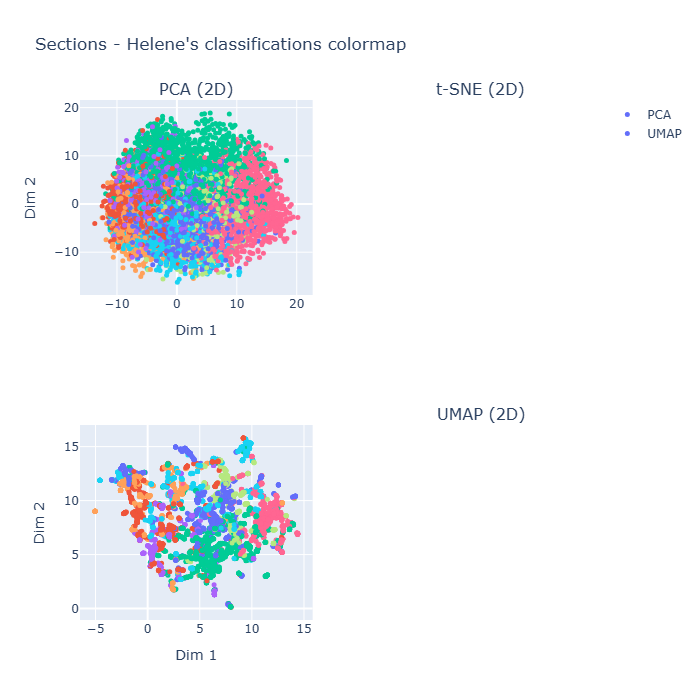
\includegraphics[width=\textwidth]{media/helene_themes.png}
        \caption{Sections colored by article theme (from Lane's analysis).}
        \label{fig:helene_themes}
    \end{subfigure}
    \hfill
    \begin{subfigure}[b]{0.49\textwidth}
        \centering
        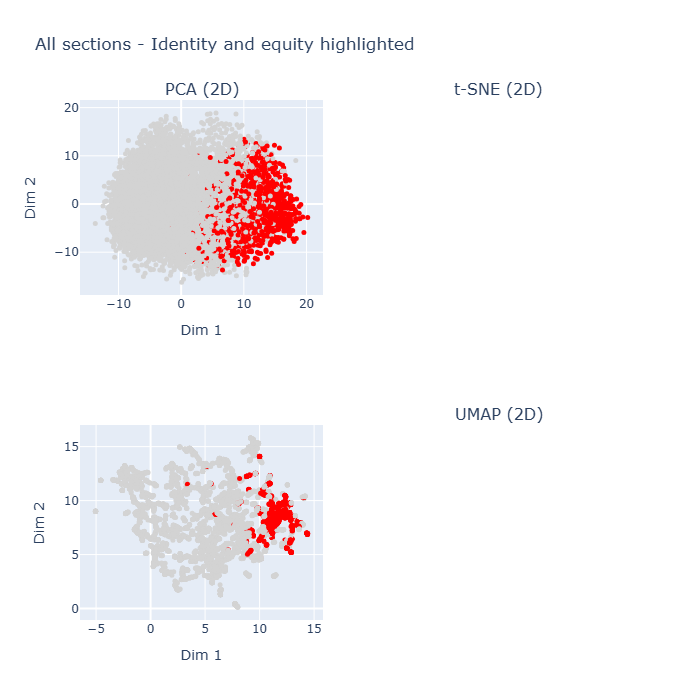
\includegraphics[width=\textwidth]{media/helene_identity_equity.png}
        \caption{Sections from "identity and equity" articles highlighted.}
        \label{fig:identity_highlight}
    \end{subfigure}
    \caption{PCA and UMAP plots of embedded sections, showing strong clustering by article theme.}
    \label{fig:pca_umap_sections}
\end{figure}

Next, we investigated the internal structure within articles.
Figure~\ref{fig:sampled_articles} shows a PCA plot of all sections, with
sections from 9 randomly sampled articles highlighted. While sections from the
same article cluster together, there is meaningful variation between them. This
\emph{intra-article spread} gives us hope that we can exploit this structure for
classification.

\begin{figure}
    \centering
    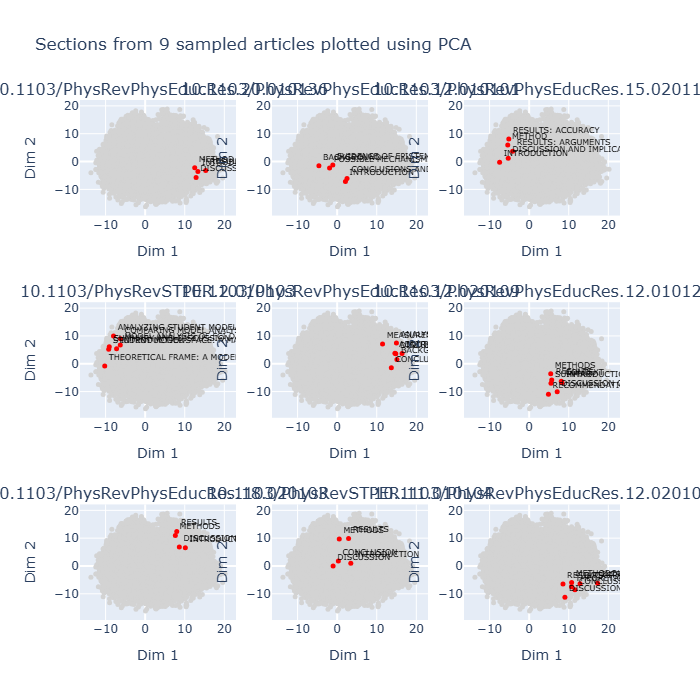
\includegraphics[width=0.7\textwidth]{media/article_sections_structure.png}
    \caption{PCA reduction of all sections with 9 randomly sampled articles highlighted.}
    \label{fig:sampled_articles}
\end{figure}

Finally, we attempted to find natural groupings based on section type using
clustering algorithms (K-Means and HDBSCAN), shown in
Figure~\ref{fig:clustering_comparison}. While the algorithms produced clusters,
these groupings did not correspond to discernible section types. This finding
underscores the \emph{need for more sophisticated, supervised classification
methods}, which we explore in the following section.

\begin{figure}
    \centering
    \begin{subfigure}[b]{0.46\textwidth}
        \centering
        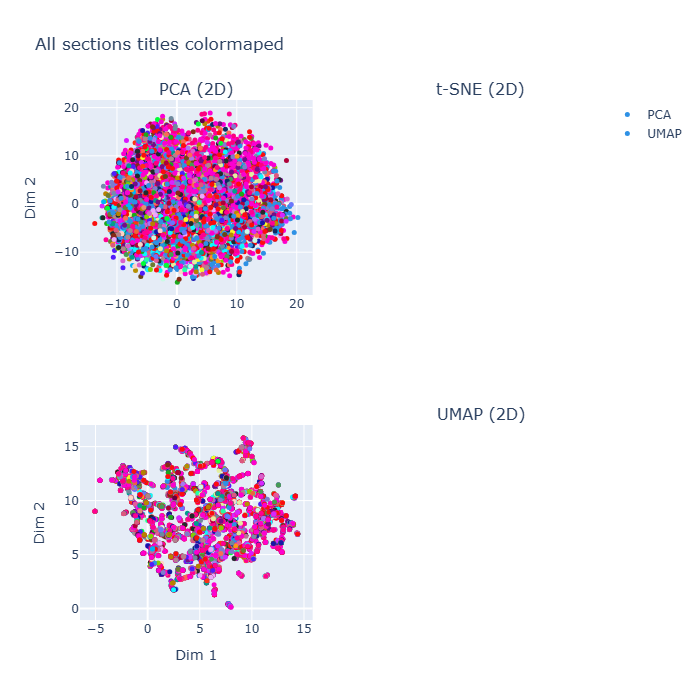
\includegraphics[width=\textwidth]{media/image4.png}
        \caption{K-Means clustering.}
        \label{fig:kmeans_cluster}
    \end{subfigure}
    \hfill
    \begin{subfigure}[b]{0.46\textwidth}
        \centering
        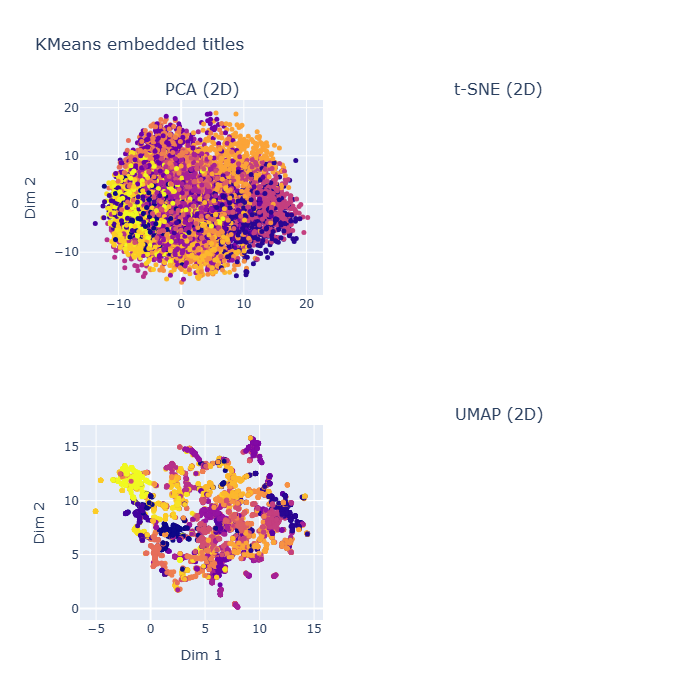
\includegraphics[width=\textwidth]{media/image5.png}
        \caption{HDBSCAN clustering.}
        \label{fig:hdbscan_cluster}
    \end{subfigure}
    \caption{A comparison of clustering algorithms applied to section embeddings. The resulting clusters did not align with section types.}
    \label{fig:clustering_comparison}
\end{figure}

\subsection{Summary of Exploratory Findings}

Our initial exploration of the section embeddings yielded three crucial insights
that shaped the subsequent direction of this project.

First, and most importantly, we found that the \emph{overarching theme of an
article is the dominant factor} determining the location of its sections in the
embedding space. Sections from articles about ``quantum physics'' cluster
together, far from sections from articles about ``identity and equity''. This
presents a significant challenge, as the thematic signal could easily overwhelm
the more subtle signal of a section's function when attempting to classify
section types.

Second, despite this strong thematic clustering, we observed a \emph{meaningful
intra-article structural variance}. Sections within the same article are not
identical points; they occupy a distinct region in the space, which suggests
that their different functions can potentially be distinguished. This finding
provides the basis for our project's feasibility.

Finally, our attempts to use unsupervised clustering algorithms to automatically
group sections by type (e.g., all `Methods` sections) were unsuccessful. This
demonstrates that while structural differences exist, they are not easily
separable.

This conclusion motivates the work of the following chapter, where we develop
and evaluate supervised models specifically designed for this classification
task.

% !TEX root = rapport_root.tex
\section{Section Type Classification}

To analyze theoretical and methodological trends in the PRPER corpus, we first
had to classify each of the 7313 sections by its section type. Since many
sections have ambiguous or non-standard headings, a simple keyword search is
insufficient. We therefore developed and evaluated several classification
methods.

This section details that process. First, we describe the benchmark dataset used
to evaluate performance. Second, we present the different classification models
we tested: a simple weighted heuristic method, a fine-tuned BERT model, and a
large language model (LLM) approach using the OpenAI API. Finally, we discuss
the trade-offs between these methods and justify our choice of model for the
subsequent analysis.

\subsection{Benchmarking}

To make meaningful judgments about the accuracy of each approach, we generated
two labeled benchmarks. The main dataset was generated by sampling 22 articles
with a total of 127 sections and hand-labeling them by their type. This provided
a representative, albeit small, set of sections covering a broad range of types.

To supplement this, we generated a larger secondary dataset of approximately 500
sections by selecting those with unambiguous headings (e.g., "Methods,"
"Introduction"). While this set is easier to classify, it allowed us to test our
models on a more robust number of samples. For evaluation, we developed a
function to compute overall accuracy, per-category metrics, and a confusion
matrix to diagnose errors.


\subsection{Classification with Heuristics}

As a baseline, we developed a simple heuristic classifier. We expected that a
section's type could be inferred from features like keywords in its title,
keywords in its content, its relative length, and its position within the
article. We combined these features into a weighted function to predict the
section type. After tuning, we found that the section title was by far the most
powerful predictor, with an optimal weight of 0.8. The heavy reliance on this
single feature indicates that other signals like section content or length were
not, on their own, strong predictors. Consequently, while this heuristic model
performs reasonably on sections with standard headings (e.g., "Introduction,"
"Methods"), it is inherently brittle and fails when encountering the many
sections with more creative or non-standard titles.


% !TEX root = rapport_root.tex
\subsection{Fine-tuned SciBERT LLM}
\subsubsection{Implementation}
To evaluate the effectiveness of transformer-based language models for scientific section classification, we fine-tune SciBERT on a subset of our dataset. To construct a high-confidence training/testing dataset, sections were grouped based on title (see \cref{tab:101}), resulting in subset of 2046 samples spread equally over 6 separate classes.
\begin{table}[h!]
\centering
\begin{tabular}{|c|l|}
\hline
\textbf{Label ID} & \textbf{Section Titles (Canonical Variants)} \\
\hline
0 & INTRODUCTION \\
\hline
1 & METHODS, METHODOLOGY, METHOD \\
\hline
2 & DATA AND RESULTS, RESULTS, FINDINGS \\
\hline
3 & DISCUSSION, DISCUSSION AND CONCLUSIONS \\
\hline
4 & CONCLUDING REMARKS, CONCLUSION, CONCLUSIONS \\
\hline
5 & THEORY, BACKGROUND, THEORETICAL FRAMEWORK, \\
  & THEORETICAL BACKGROUND, LITERATURE REVIEW \\
\hline
\end{tabular}
\caption{Canonical section title groups used for high-confidence label assignment.}
\label{tab:101}
\end{table}

Fine-tuning was implemented with the Huggingface Transformers library, initializing the model using the 'allenai/scibert\_scivocab\_uncased' checkpoint and 'AutoModelForSequenceClassification' class. Tokenization was handled using the corresponding 'AutoTokenizer', truncated to a maximum of 512 tokens and padded to ensure homogeneous data length. Since we are only doing transfer learning, the embedding and encoder model layers were frozen, relying on iterative adjustment of the final pooler layers to aggregate model output into an interpretable classification output vector. The final model was optimized using a 30-35-35 training-testing-validation-split to minimize overfitting, with hyperparameters
$$
l_r = 2\cdot 10^{-4}, \quad \text{Batch Size} = 8, \quad \text{Epochs} = 10.
$$
(see notebook 'bert\_section\_classifier.ipynb' for full implementation)
\subsubsection{Results and Discussion}
The model was trained locally on an NVIDIA GPU over the span of $\sim$7 hours. Key training and evaluation metrics (summarized in \cref{tab:102}) show a steady decrease in training and evaluation loss from 1.3488 and 1.0107 after the first epoch to 0.5358 and 0.5754 after epoch 10, respectively. Model accuracy on evaluation data showed a corresponding increase from 0.638 to 0.769 during the same period, suggesting that the model is learning generalizable patterns rather than overfitting to the data. Notably, the metrics also show a clear plateau around epoch 7-8, suggesting that further mode convergence does not result in any noticable performance improvements. Reducing training to 8 epochs may therefore save time and computational resources without adversely affecting model classification capabilities.

\begin{table}[h!]
\centering
\begin{tabular}{|c|c|c|c|c|c|}
\hline
\textbf{Epoch} & \textbf{Train Loss} & \textbf{Eval Loss} & \textbf{Eval Accuracy} & \textbf{Learning Rate} & \textbf{Grad Norm} \\
\hline
1  & 1.3488 & 1.0107 & 0.638 & 1.80e-4 & 5.63 \\
2  & 0.9062 & 0.8415 & 0.668 & 1.60e-4 & 5.11 \\
3  & 0.7612 & 0.7020 & 0.717 & 1.40e-4 & 4.19 \\
4  & 0.6701 & 0.6754 & 0.746 & 1.20e-4 & 6.02 \\
5  & 0.6338 & 0.6465 & 0.749 & 1.00e-4 & 3.16 \\
6  & 0.6026 & 0.6249 & 0.752 & 8.01e-5 & 3.58 \\
7  & 0.5862 & 0.6030 & 0.772 & 6.01e-5 & 3.16 \\
8  & 0.5716 & 0.5855 & 0.772 & 4.01e-5 & 3.72 \\
9  & 0.5560 & 0.5835 & 0.765 & 2.01e-5 & 3.34 \\
10 & 0.5358 & 0.5754 & 0.769 & 1.12e-7 & 5.54 \\
\hline
\end{tabular}
\caption{Training and evaluation metrics for SciBERT across 10 epochs.}
\label{tab:102}
\end{table}

\Cref{tab:103} presents model evaluation on validation data. Overall accuracy was found to be 0.772. The precision and recall of 0.791 and 0.772, respectively, and the resulting F1-score of 0.776, indicate balanced false-positive and false-negative across the classes. The log loss of 0.646 suggests relatively high model confidence when making correct choices and large uncertainty when making incorrect ones. This is further reinforced by an average confidence of 0.750 and average entropy of 0.645, implying (generally) sharply focused model prediction with low uncertainty and diffuseness. Examining \Cref{tab:104} and \Cref{fig:101} reveals average model performance on sections "Introduction", "Conclusion" and "Discussion", with higher predictive ability on sections "Methods" and "Results" and a rather lackluster F1-score of 0.629 on "Theory" sections. \Cref{fig:101} indicates that this performance drop is a concequence of frequent misclassification of "Theory" sections as "Introduction", and vice versa. Interestingly, the matrix shows elevated numbers for diagonal-adjacent tiles, suggesting that false label assignments primarily occur between "bordering" article sections. This hints at the fact that articles trace a continuous "semantic path" from beginning to end, resulting in textually adjacent sections being more closely related (and therefore harder to distinguish). We will explore this characteristic more thoroughly in later analysis.

\begin{table}[ht]
\centering
\caption{Overall Evaluation Metrics on Validation Data}
\begin{tabular}{lcc}
\toprule
\textbf{Metric} & \textbf{Value} \\
\midrule
Accuracy               & 0.772 \\
Precision   & 0.791 \\
Recall      & 0.772 \\
F1-score    & 0.776 \\
Log Loss               & 0.646 \\
Average Confidence     & 0.750 \\
Average Entropy        & 0.645 \\
\bottomrule
\end{tabular}
\label{tab:103}
\end{table}

\begin{table}[ht]
\centering
\caption{Per-Class Evaluation Metrics}
\begin{tabular}{lcccc}
\toprule
\textbf{Class} & \textbf{Precision} & \textbf{Recall} & \textbf{F1-score} & \textbf{Support} \\
\midrule
Introduction          & 0.759 & 0.721 & 0.739 & 61 \\
Theory                & 0.550 & 0.733 & 0.629 & 45 \\
Methods               & 0.933 & 0.808 & 0.866 & 52 \\
Results               & 0.785 & 0.911 & 0.843 & 56 \\
Discussion            & 0.809 & 0.731 & 0.768 & 52 \\
Conclusion            & 0.906 & 0.707 & 0.795 & 41 \\
\bottomrule
\end{tabular}
\label{tab:104}
\end{table}

\begin{figure}%[h!]
    \centering
    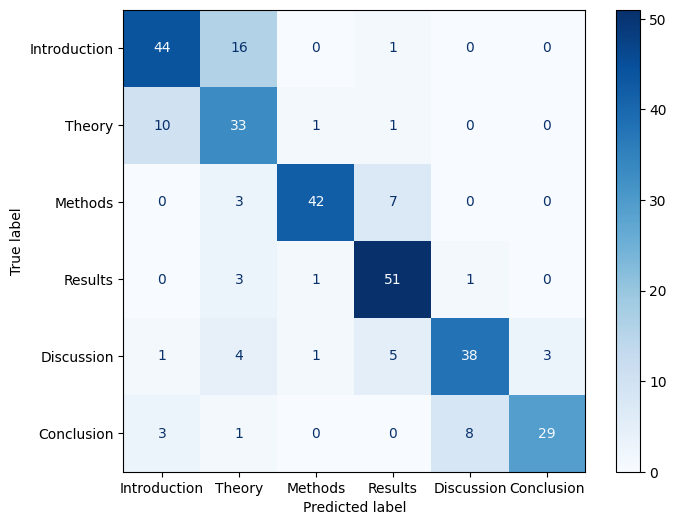
\includegraphics[width=.6\linewidth]{media/transformer_confusion_matrix.png}
    \caption{Confusion Matrix outlining model performance on validation split.}
    \label{fig:101}
\end{figure}

\subsection{Projection Based Classification}
While fine-tuning a language model is effective, it is often computationally demanding, time-consumimg, and unecessary complex for simple og low-resource applications. Leveraging the geometric properties of textual embeddings, we iteratively develop and implement a lightweight classification approach that offers a fast, interpretable and data-efficient alternative to full fine-tuning. To maintain alignment with prior benchmarks, we rely on the same six-category classification dataset as used in SciBERT fine-tuning. All data are encoded using the text-embedding-3-large model from OpenAI.

\subsubsection{Implementation}
\paragraph{Mean Embedding Similarity}
Given a small number of labeled samples per class, we calculate class wise means represent the prototypical embedding of each class in the semantic space. These mean vectors serve as centroids, or "semantic signatures", and summarize the contextualized representations of each class. The similarity of a given sample $x$ to a given class is calculated using the inner product
\begin{equation}
    \text{sim}(x, \mu_{c}) = \braket{x, \mu_c}
\end{equation}
where $\mu_c$ is the respective, normalized, class mean. The resulting score can be interpreted as a measure of sample-class alignment. Returning to the data-subset used for fine-tuning previously, we create a new dataframe containing only instances of "Introduction" and "Results" (arbitrarily chosen). Calculating an "Introduction" mean, we associate a score with each sample using (1). Sorting the data by this score, we see a clear class seperation (see \cref{fig:102} (2)).

\begin{figure}%[H]
    \centering
    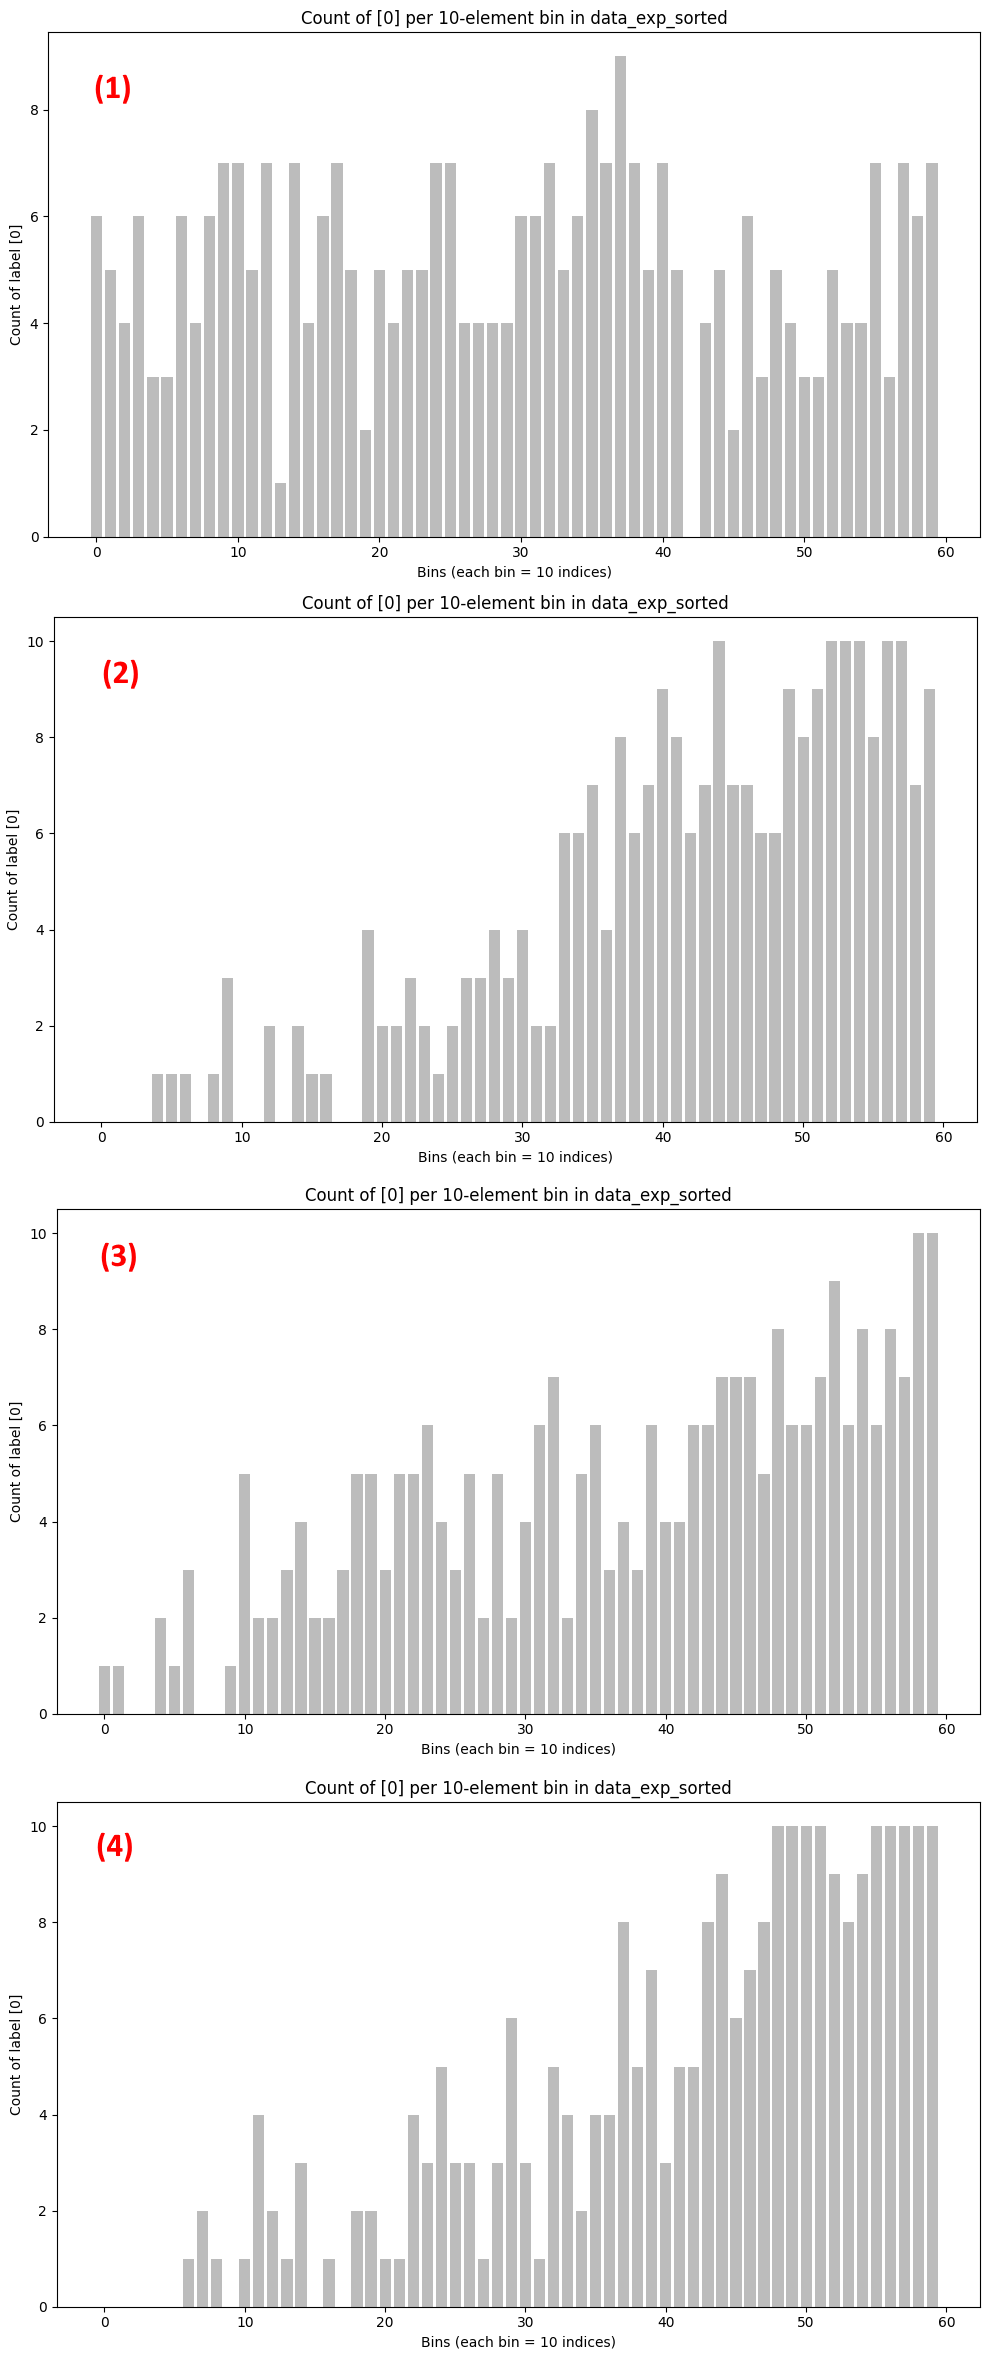
\includegraphics[width=0.5\linewidth]{media/score_sorting.png}
    \caption{Distribution of labels in dataset. A bin along the x-direction represent a 10 consecutive data entries, with the number along the y-axis indicating percentage of label 0 among the entries.}
    \label{fig:102}
\end{figure}

\paragraph{Class-centroid Difference Scoring}
Given last paragraphs inerpretation of class centroids as being prototypical representation of each class, it seems intuitive that the difference vector $v = \mu_2-\mu_1$ between two class centroids $\mu_{1}$ and $\mu_{2}$ should somehow "encode" the semantic difference between the classes. In other words, $v$ captures how the meaning of class 1 diverges from that of class 2 in the embedding space. It might therefore also be interesting to get a measure of where a sample embedding falls along this seperation axis. For any sample $x$, we take its projection onto the centroid difference vector (see \cref{fig:103})
\begin{equation}
    \text{proj}_{v}(x) = \frac{\braket{x, v}}{\braket{v, v}}v = \braket{x, v}v = k\cdot v, \quad k = \braket{x, v}
\end{equation}
where we assume that the difference vector $v$ has already been normalized $|v| = 1$. In the end result $v$ is independent of $x$, and we are left with the inner product $k$ being the metric of interest, indicating the position of a sample projection along the seperation axis, ranging from $k = -\infty$ (really far in direction of Class 1) to $k = \infty$ (really far in direction of Class 2).
\begin{figure}%[h]
    \centering
    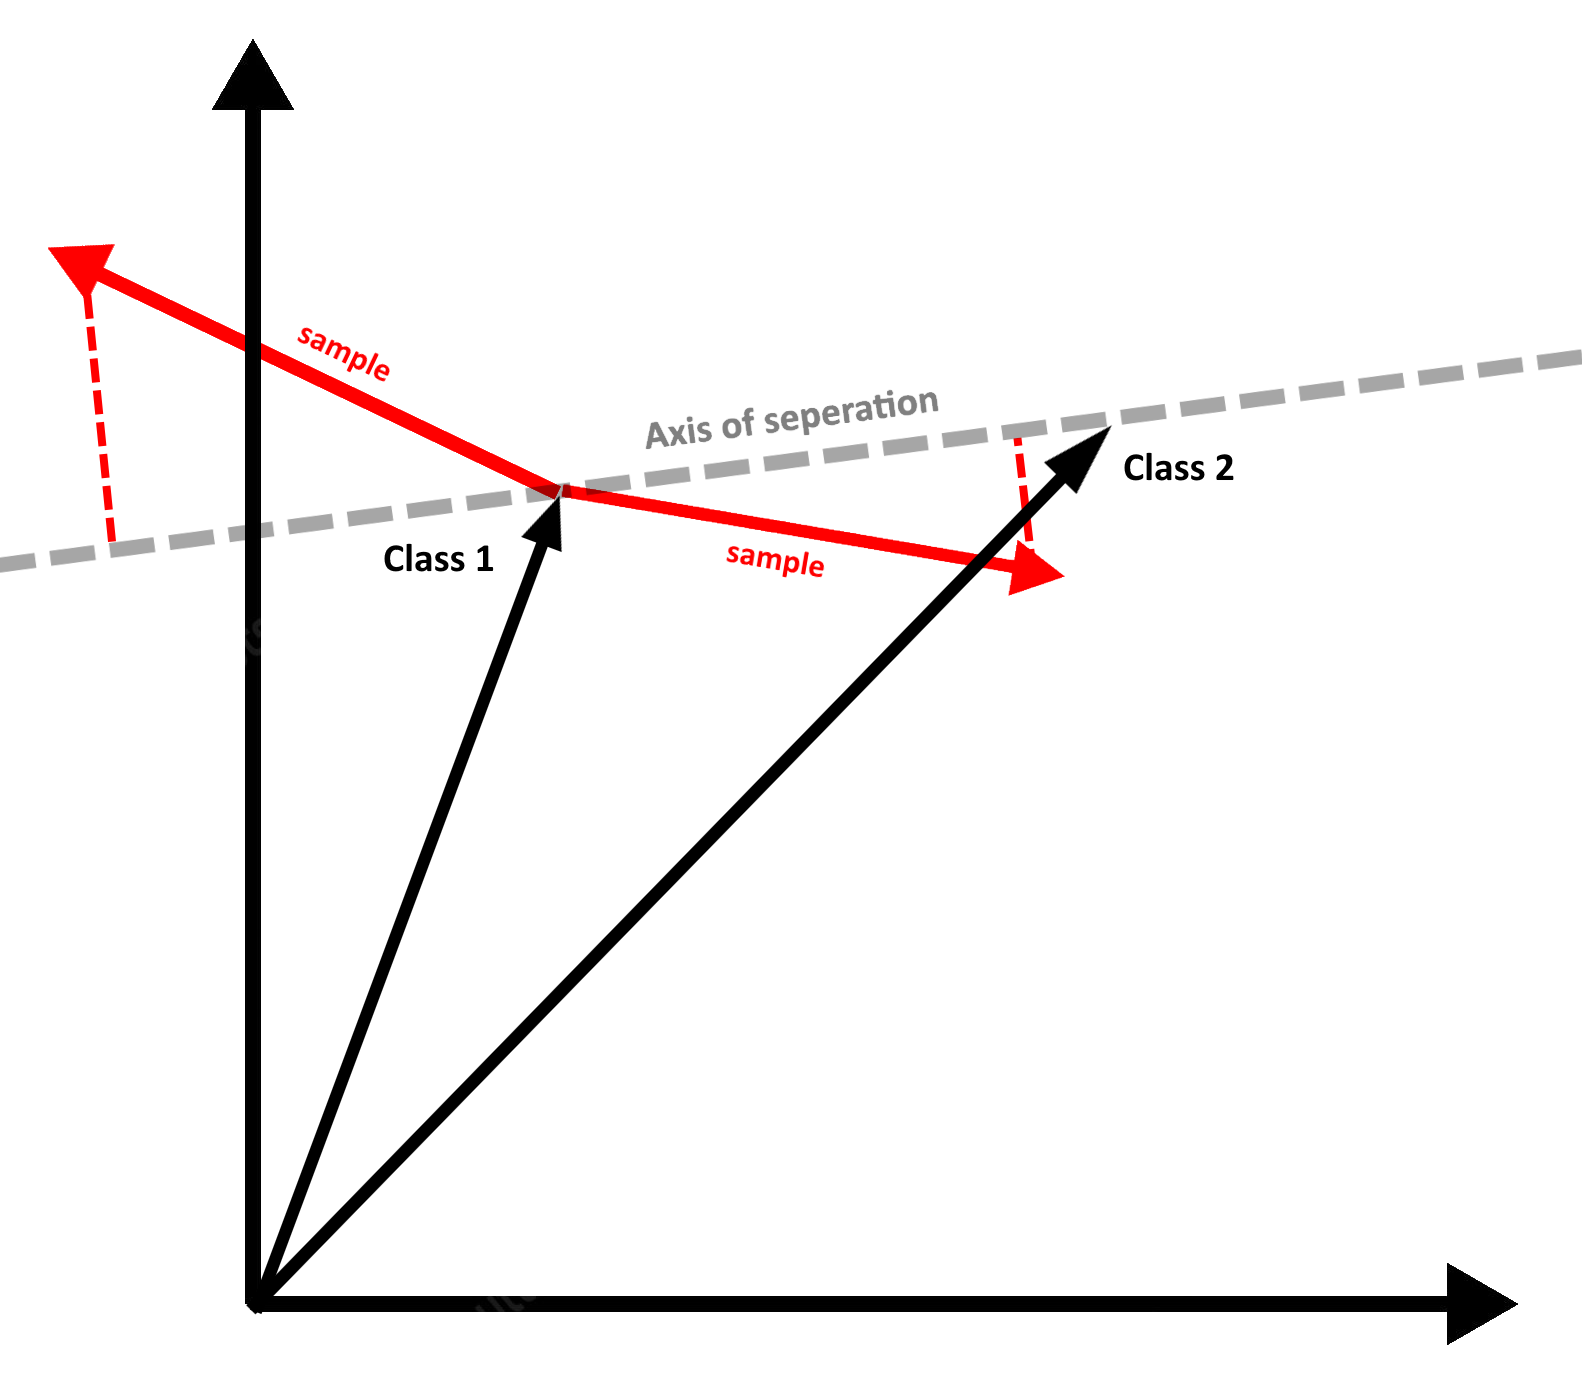
\includegraphics[width=0.5\linewidth]{media/vec_diff_graphic.png}
    \caption{Geometric visualization of the centroid difference vector and the projection upon it.}
    \label{fig:103}
\end{figure}
In the end we are left with a "seperation" score
\begin{equation}
    \text{sep}(x, v =\mu_{c2}-\mu_{c1}) = \braket{x, v}
\end{equation}
Testing again on the aforementioned "Introduction/Results" dataset, we calculate a centroid difference vector and associate a "seperation" score with each sample. Sorting the data by this score, we again see a clear class seperation (see \cref{fig:102} (3)).
\paragraph{Combined Scores and Binary Model Implementation}

These scores are in a sense complementary, with "similarity" scores measuring sample alignment with centroids and "seperation" scores measuring sample-centroid displacement. Combining the two into a single, combined, score
\begin{equation}
    \text{score} = \lambda \cdot \text{sim}(x, \mu_{c1})+(1-\lambda)\cdot \text{sep}(x, \mu_{c2}-\mu_{c1})
\end{equation}
where score weighting is adjusted by varying $\lambda$. Arbitrarily choosing $\lambda = 0.5$ and sorting the same data as before by this new score, we seemingly obtain the best class separation yet (\Cref{fig:102} (4)). Using this combined score, we implement a binary classification model and test it on all $\begin{pmatrix}
    6\\
    2
\end{pmatrix}$ binary 6-class combinations (still testing on the same 2046-sample dataset used previously) using a 0.7/0.3 train-test-split. The decision threshold for assigning binary labels is defined as the median of the score distribution. We also evaluate model performance on the training split for a range of $\lambda\in[0, 1]$ to find optimal score-weighting.

\begin{table}[ht]
\centering
\caption{Summary of Binary Classification Metrics Across All Class Pairs}
\begin{tabular}{lcccc}
\toprule
\textbf{Statistic} & \textbf{Accuracy} & \textbf{Precision} & \textbf{Recall} & \textbf{F1-score} \\
\midrule
\textbf{Mean}   & 0.902             & 0.904              & 0.900           & 0.901 \\
\textbf{Maximum}   & 0.976             & 0.989              & 0.990           & 0.974 \\
\textbf{Minimum}   & 0.732             & 0.755              & 0.705           & 0.729 \\
\bottomrule
\end{tabular}
\label{tab:105}
\end{table}

\noindent \Cref{tab:105} shows a generally strong and balanced model performance above 0.900 across the board, with maximum performance in the high 0.900s. Introduction/Theory classification is however an outlier, with values in the low 0.700s. This comes as no suprise given our previous findings with the fine-tuned SciBERT model.


(see notebook "nonMLP\_classifier.ipynb" for full implementation)
\subsubsection{Full Multi-Class Classification Model}

\paragraph{Non-MLP Implementation}

Multi-class classification ability is handled using a One-vs-One (OvO) approach, which involves fitting a distinct binary classifier to all $\begin{pmatrix}
    n_{\text{classes}}\\
    2
\end{pmatrix}$ class combinations. Each binary classifier in the ensemble operates using the lightweight scoring approach outlined above, calculating class means, combined scores according to (4), with individually optimized $\lambda$-weighting. When applied to a sample, each constituent classifier casts a binary vote, and final model prediction is aggregated using a majority vote. The model was fitted to the data, taking sub-5 seconds. It was then evaluated on the test split using key metrics, presented in \Cref{tab:106}, \Cref{tab:107} and \Cref{fig:104}.

\begin{table}%[ht]
\centering
\caption{Overall Evaluation Metrics for Non-MLP Classifier}
\begin{tabular}{lr}
\toprule
\textbf{Metric} & \textbf{Value} \\
\midrule
Accuracy            & 0.713 \\
Precision & 0.715 \\
Recall    & 0.713 \\
F1-score  & 0.713 \\
Log Loss             & 1.275 \\
Average Confidence   & 0.331 \\
Average Entropy      & 1.494 \\
\bottomrule
\end{tabular}
\label{tab:106}
\end{table}

\begin{table}%[ht]
\centering
\caption{Per-Class Evaluation Metrics}
\begin{tabular}{lcccc}
\toprule
\textbf{Class} & \textbf{Precision} & \textbf{Recall} & \textbf{F1-score} & \textbf{Support} \\
\midrule
Introduction      & 0.568 & 0.636 & 0.600 & 118 \\
Methods           & 0.867 & 0.875 & 0.871 & 104 \\
Results           & 0.787 & 0.842 & 0.813 & 101 \\
Discussion        & 0.646 & 0.634 & 0.640 & 101 \\
Conclusion        & 0.767 & 0.702 & 0.733 & 94  \\
Theory            & 0.679 & 0.594 & 0.633 & 96  \\
\bottomrule
\end{tabular}
\label{tab:107}
\end{table}

\begin{figure}%[ht]
    \centering
    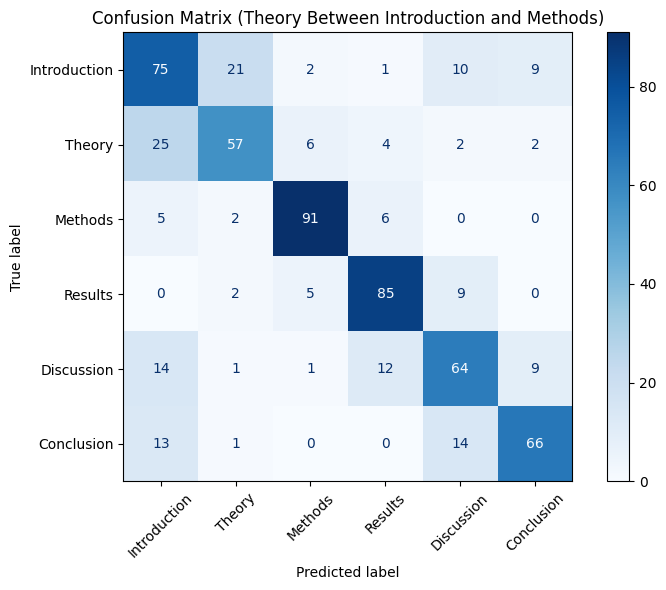
\includegraphics[width=0.6\linewidth]{media/nonML_confusion_matrix.png}
    \caption{Confusion Matrix outlining non-MLP model performance on test split.}
    \label{fig:104}
\end{figure}
\noindent (see notebook 'nonMLP\_classifier.ipynb' for full implementation)
\paragraph{MLP Implementation}
To further enhance model performance, we replace the majority voting system with a multi-layer perceptron (MLP), trained to map the combined projection scores to class logits. Using the same OvO-approach, the resulting scores are fed into an MLP with input dimensions $2\cdot \begin{pmatrix}
    n_{\text{classes}}\\
    2
\end{pmatrix}$. That is, weighting using the aforementioned $\lambda$ is discarded in favour of directly inputting all scores into the neural network. The input layer is succeeded by three ReLU-activated hidden layers, gradually consolidating the input into fewer dimensions, resulting finally in an output layer producing a single logit for each class.

%\Testing % @Lars, what is this?
for a range of different hyperparameters (see notebook 'mlp\_classifier.ipynb' for more details), optimal performance on the data was found for the following parameters
$$l_r = 5\cdot 10^{-4}, \quad \text{Hidden Layer Dimensions} = [32, 16, 8], \quad \text{Epochs} = 200.$$

Model fitting completed in under 10 seconds. Resulting model performance is outlined in \Cref{tab:108}, \Cref{tab:109}, \Cref{tab:110} and \Cref{fig:105}.

\begin{figure}%[ht]
    \centering
    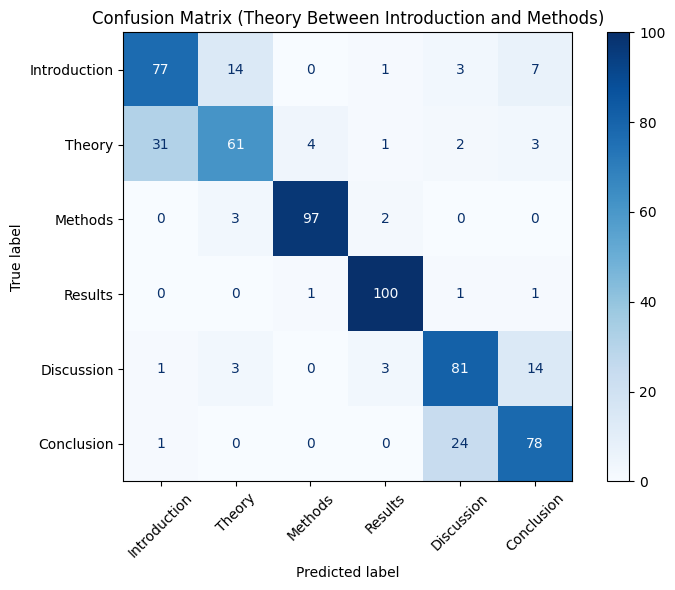
\includegraphics[width=0.6\linewidth]{media/MLP_confusion_matrix.png}
    \caption{Confusion Matrix outlining MLP model performance on test split.}
    \label{fig:105}
\end{figure}
\begin{table}[ht]
\centering
\caption{Summary of Binary Classification Metrics}
\begin{tabular}{lcccc}
\toprule
\textbf{Statistic} & \textbf{Accuracy} & \textbf{Precision} & \textbf{Recall} & \textbf{F1-score} \\
\midrule
Average & 0.902 & 0.903 & 0.905 & 0.903 \\
Maximum & 0.985 & 0.991 & 1.000 & 0.986 \\
Minimum & 0.751 & 0.737 & 0.771 & 0.767 \\
\bottomrule
\end{tabular}
\label{tab:108}
\end{table}

\begin{table}[ht]
\centering
\caption{Overall Evaluation Metrics for MLP Classifier}
\begin{tabular}{lc}
\toprule
\textbf{Metric} & \textbf{Value} \\
\midrule
Accuracy               & 0.805 \\
Precision   & 0.804 \\
Recall     & 0.805 \\
F1-score    & 0.803 \\
Log Loss               & 0.529 \\
Average Confidence     & 0.786 \\
Average Entropy        & 0.552 \\
\bottomrule
\end{tabular}
\label{tab:109}
\end{table}

\begin{table}[ht]
\centering
\caption{Per-Class Evaluation Metrics for MLP Classifier}
\begin{tabular}{lcccc}
\toprule
\textbf{Class} & \textbf{Precision} & \textbf{Recall} & \textbf{F1-score} & \textbf{Support} \\
\midrule
Introduction & 0.700 & 0.755 & 0.726 & 102 \\
Theory & 0.753 & 0.598 & 0.667 & 102 \\
Methods & 0.951 & 0.951 & 0.951 & 102 \\
Results & 0.935 & 0.971 & 0.952 & 103 \\
Discussion & 0.730 & 0.794 & 0.761 & 102 \\
Conclusion & 0.757 & 0.757 & 0.757 & 103 \\
\bottomrule
\end{tabular}
\label{tab:110}
\end{table}


\subsubsection{Model Comparison and Discussion}
The projection classification model offer a lightweight alternative to full fine-tuning. From \Cref{tab:105}, \Cref{tab:106} and \Cref{tab:107} we see that the non-MLP variant performs well on binary classification tasks (both accuracy and F1 score above 0.9), but multi-class classification performance is significantly worse (accuracy and F1-score of 0.713) class wise performance even lower (F1-score of 0.600) on "Introduction" sections. Looking at \Cref{fig:104} it is evident that the model suffers from the same diagonal-adjacent class mislabeling, but in addition it also frequently misclassifies "Introductions" as "Discussion/Conclusion" and vice versa. The implementation also suffers from a large flaw; the decision threshold from label assignment is based on the median of the score distribution. This results in a model that is extreme sensitive to class imbalances in the training split. To examine this we test binary classification performance on "Introduction" and "Methods" sections for differing label imbalances. A 1:1 label relation results in a classification performance of $\sim$0.95. This number decreases to $\sim$0.84 for a label imbalance of 2:1, and increasing the discrepancy to 4:1 results in a performance drop to $\sim$0.73.


The MLP-approach replaces this fixed threshold strategy with a trainable component capable of learning non-linear relationships between class score-pairs. \Cref{tab:108} shows that this does not seem to increase binary classification performance, with very little improvement in mean (though minimum performance does increase from an F1-score 0.729 to 0.767). Comparing \Cref{tab:106} and \Cref{tab:109} shows significant improvements in multi-class performance, with accuracy and F1-scores increasing from 0.713 and 0.713 to 0.805 and 0.803, respectively. Average model confidence also increase by almost 2.5x, while average entropy is cut by 2/3 the original value (though these gains do come at the cost of intuitiveness/interpretability). Looking at \Cref{fig:105} we see that misclassifications are now limited almost completely to "Introduction/Theory" and "Discussion/Conclusion". We also tried to train several MLPs in parallel, mimicking a sort of weak learning approach, with final output being the mean of all estimators. Testing for $n_{\text{estimators}}\in [1, 2, 4, 8, 16]$ over a range of hyperparameters, we saw very-slight to nonexistent performance improvements ($\sim 1\%$) on our data, indicating that this does not yield any significant advantage.


Comparing these projection models with the fine-tuned SciBERT model we see that the MLP-variant outperforms the fine-tuned LLM, with higher accuracy (0.805 v. 0.772), F1-score (0.803 v. 0.776), higher confidence (0.786 v.0.750) and lower entropy (0.552 v. 0.645). While not as fast as the non-MLP model (sub 5-second training time), the MLP model delivers performance rivaling the fine-tuned LLM at a fraction of the computational cost and time (sub 10-second v. $\sim$7hrs). It is also more data-efficient (though the MLP-variant is less so), primarily utilizing few shot sampling of 8 examples per class. \Cref{fig:106} shows that the means calculated using $n$ samples converges to the global mean using all samples very quickly, suggesting that sampling only a few examples does not significantly impact performance. Testing on the models reflects this fact; increasing the number pof samples $n$ results only in very slight performance gains ($\sim$1\%) on our data. This indicates that these projection models are a lightweight alternative to full-on model fine-tuning, offering competitive performance with greatly improved computational- and data efficiency.

\begin{figure}%[h!]
    \centering
    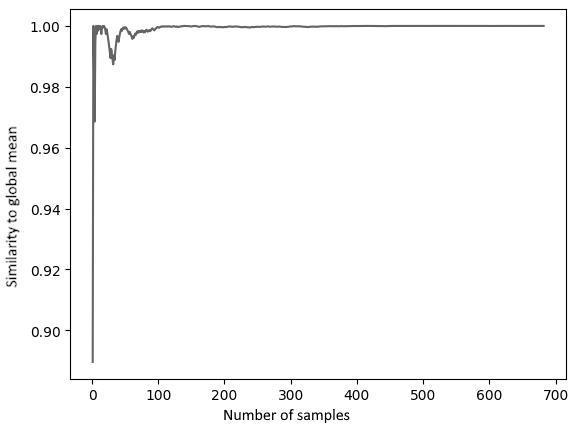
\includegraphics[width=0.7\linewidth]{media/few_shot_sampling.png}
    \caption{Inner product of normalized average of $n$ embeddings with global average. We see that it quickly approaches 1.}
    \label{fig:106}
\end{figure}


While these projection models do not utilize computationally intensive transformers, they depend on the existence of high quality embedding models. In fact, the models are very sensitive to the quality of the embeddings. The data, instead embedded using the 'Voyager-3-large' embedding model, immediately causes a sharp performance drop of $\sim 7\%$ (relative). This approach is lightweight and quick only if embeddings are precomputed; in other words, it is still implicitly dependent on large, compute- and data hungry models, leading the real computational cost to be much higher than these results give the impression of. This juxtaposition risks completely invalidating the model’s original motivation and conceptual justification. It also raises another important point; while the projection models utilize cutting-edge, modern embedding models, the SciBERT implementation uses its own aging tokenizer, perhaps resulting in lower quality input and thereby rendering the comparison between the two unfair and biased.

\subsubsection{2D visualization of score-pairs}
Visualizing these score pairs seems an interesting prospect, perhaps yielding some new insight or intuition. Returning to the same dataset as earlier, we calculate the global mean embedding and the difference vector between the "Introduction"- and "Conclusion" mean centroids. Finding the aforementioned "similarity" and "seperation" scores of all section samples and plotting them as 2-dimensional points (\Cref{fig:107}), we see clear clustering on a section-type basis. What is perhaps most interesting is how this contrasts with earlier findings; using other dimensional-reduction techniques, sections seemed to display thematically based clustering. This plot seems to indicate the opposite (perhaps this is caused by the fact that the specially selected "Introduction/Conclusion" difference vector specifically "picks out" the sample-embedding characteristics most similar to its own?). Instead plotting the means of $\sim$20 embeddings on a class by class basis (attempting to reduce semantic noice), we see a clear seperation of classes (see \Cref{fig:108}). 

\begin{figure}%[H]
    \centering
    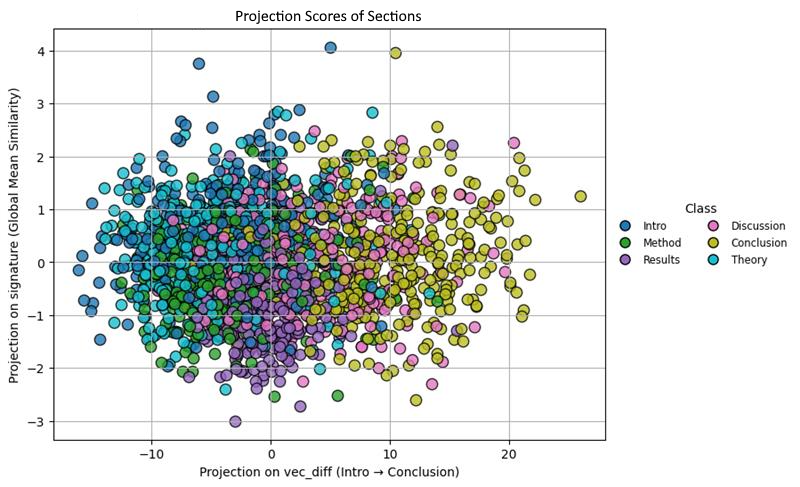
\includegraphics[width=.8\linewidth]{media/section_projections.png}
    \caption{2D projection scores of sections onto Introduction/Conclusion difference vector (x-axis) and global average embedding (y-axis).}
    \label{fig:107}
\end{figure}


Interestingly, the clusters trace out the semantically logical path from "Introduction" to "Conclusion" along the x-axis, indicating that the "Intro/Conclusion" difference vector seemingly captures the entire semantic path of the article from beginning to end, with "Introduction" and "Conclusion" at each side, "Theory" and "Methods" very similar to "Introduction", and "Results" and "Discussion" progressively moving towards the right. The y-axis also shows "Introductions" as being the most similar to the global mean and "Results" as being the most divergent. Furthermore, the proximity of "Introduction" and "Theory" reinforces the earlier result that the sections-classes are closely related, given that they were often mistakenly interchanged by the classification models.

\begin{figure}%[h!]
    \centering
    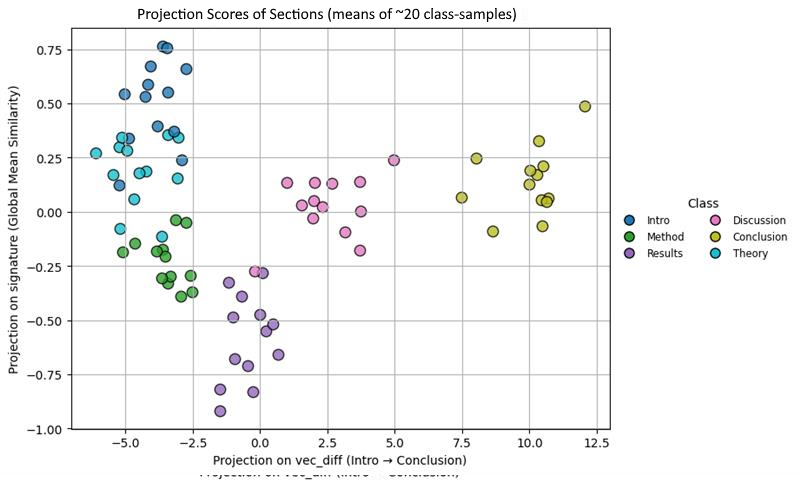
\includegraphics[width=.8\linewidth]{media/mean_section_projections.png}
    \caption{2D projection scores of mean embeddings of ~20 sections of same type onto Introduction/Conclusion difference vector (x-axis) and global average embedding (y-axis).}
    \label{fig:108}
\end{figure}

This visualization tool provides a different way of considering the projection scores, and will be used extensively during further analysis.


\subsection{Classification with Large Language Models (LLMs)}

We next tested a classification approach using OpenAI's API. After experimenting
with prompts and context, we found the most effective and efficient method was
to pass the entire text of an article at once, asking the model to return a JSON
object classifying all of its sections in a single API call. This approach was
approximately seven times faster and, in addition, more accurate than
classifying sections individually.

Using this method with the `gpt-4o` model, we achieved an accuracy of \emph{90\%}
on our hand-labeled benchmark dataset. The model achieved near-perfect accuracy
on the simpler heading-based dataset. The confusion matrix (Figure
\ref{fig:conf_matrix}) reveals that most misclassifications occur between
categories that are often conceptually similar, such as mistaking a `Theoretical
Framework` for a `Literature Review`, or confusing `Implications` with
`Conclusion`.

\begin{figure}
    \centering
    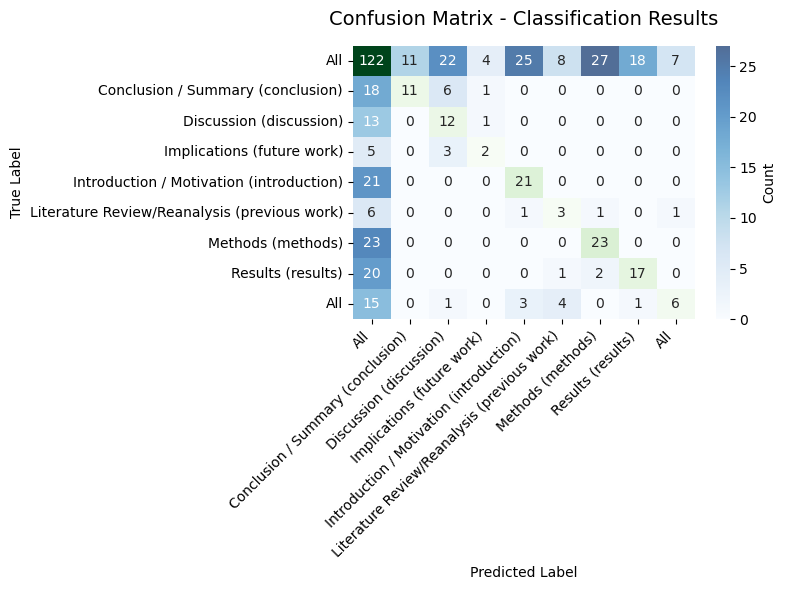
\includegraphics[width=0.9\textwidth]{media/confussion_matrix_sections.png}
    \caption{Confusion matrix for the LLM-based section classification on our hand-labeled benchmark dataset.}
    \label{fig:conf_matrix}
\end{figure}


\subsection{Discussion of Classification Methods}

Our experiments evaluated four distinct classification methods, revealing a clear trade-off between performance, computational cost, and implementation complexity. The final accuracy of each model on a comparable benchmark dataset is summarized in Table~\ref{tab:accuracy_summary}.


\begin{table}%[h!]
\centering
\caption{Classification accuracy across different methods on the hand-labeled benchmark.}
\label{tab:accuracy}
\begin{tabular}{lc}
    \toprule
    \textbf{Classification method} & \textbf{Accuracy} \\
    \midrule
    Heuristics             & $\sim$0.70 \\
    \addlinespace
    Fine-tuned SciBERT & 0.77 \\
     Projection-Based MLP & 0.80 \\
    \addlinespace
    LLM (gpt-4.1)          & $\sim$0.90 \\
    LLM (gpt-4.1-mini)     & $\sim$0.80 \\
    \bottomrule
\end{tabular}
\end{table}

The simple \emph{heuristic model} served as a useful baseline but proved too brittle for this task. Among the locally run models, the fine-tuned \emph{SciBERT} represents a standard deep learning approach, achieving a respectable accuracy of \emph{0.77}, but at the cost of significant training time ($\sim$7 hours). In contrast, our novel \emph{projection-based MLP classifier} emerged as a powerful and lightweight alternative. It not only surpassed the SciBERT model with an accuracy of 0.80 but did so with a fraction of the computational cost (training in under 10 seconds) and greater data efficiency. Its primary dependency is the availability of high-quality, pre-computed text embeddings.

Finally, the \emph{LLM-based approach} using an external API delivered the highest performance, with an accuracy of approximately \emph{$\sim$0.90}. Its main drawbacks are the monetary cost of API calls and the reliance on a closed-source service, which is unsuitable for datasets with sensitive data.

Crucially, the errors made by the top-performing models often highlight genuine ambiguity in the source material. Sections titled "Discussion and Conclusion" are conceptually overlapping, and the line between a "Literature Review" and a "Theoretical Framework" can be blurry even for a human reader. This suggests that the \emph{$\sim$0.90} accuracy achieved by the LLM is approaching the practical ceiling for this classification task with this set of discrete categories.

Given its state-of-the-art performance and our goal of obtaining the highest quality classifications for our subsequent trend analysis, we selected the \emph{LLM-based classifier} for processing the entire dataset. However, our results show that the projection-based MLP is a highly compelling local alternative, offering competitive performance with minimal computational overhead.

\subsection{Exploring Inter-Section Vector Arithmetic}

Inspired by classic word embedding analogies like `king - man + woman \approx
queen`, we briefly explored whether similar vector arithmetic could model the
transitions between section types (e.g., from `Theory` to `Methods`).
Our initial, na\"{\i}ve attempt involved calculating a 'transition vector' by
subtracting a theory section's embedding from its corresponding methods
section's embedding.

This simple implementation did not yield clearly predictive results. We suspect
this is because the powerful 'thematic signal' of an entire article can easily
obscure the more subtle 'section type signal' that defines a section's function.
While a more sophisticated approach might yet prove fruitful, a deeper
investigation of this specific technique fell outside the scope of the current
project.

% !TEX root = rapport_root.tex
\section{Content Analysis with an Iterative LLM: Identifying Theories and Methods}

Once the articles were classified into section types, we were well-poised to
perform a more fine-grained analysis. Our goal was to move beyond broad topics
and identify the specific theoretical frameworks and research methods used
within the PRPER corpus, and to track how their usage has evolved over time. To
achieve this, we developed a novel, iterative classification workflow that uses
an LLM to discover and assign fine-grained categories directly from the text.

\subsection{Methodology: An Iterative Classification Workflow}

To extract specific information like theoretical frameworks, we developed a
staged, iterative approach that uses an LLM to build a classification scheme
from the ground up. As illustrated in Figures \ref{fig:classifier_logic} and
\ref{fig:classifier_workflow}, the process involves:
\begin{enumerate}
    \item Feeding a sample of text sections to an LLM to generate an initial
    list of categories.
    \item Using this list to classify all sections.
    \item Reviewing the classifications and having the LLM refine or merge the
    categories.
    \item Repeating the process until the classification scheme is stable and
    comprehensive.
\end{enumerate}
This logic is implemented in a flexible Python `AbstractClass`. A key feature of
this implementation is the format of the LLM's response. For each section, the
model returns both a direct array of classifications (e.g., the specific
frameworks it identifies) and a corresponding probability distribution. This
provides analytical flexibility, allowing us to either accept the model's direct
classifications, filter results by a confidence threshold, or select only the
single highest-probability result.

\begin{figure}
    \centering
    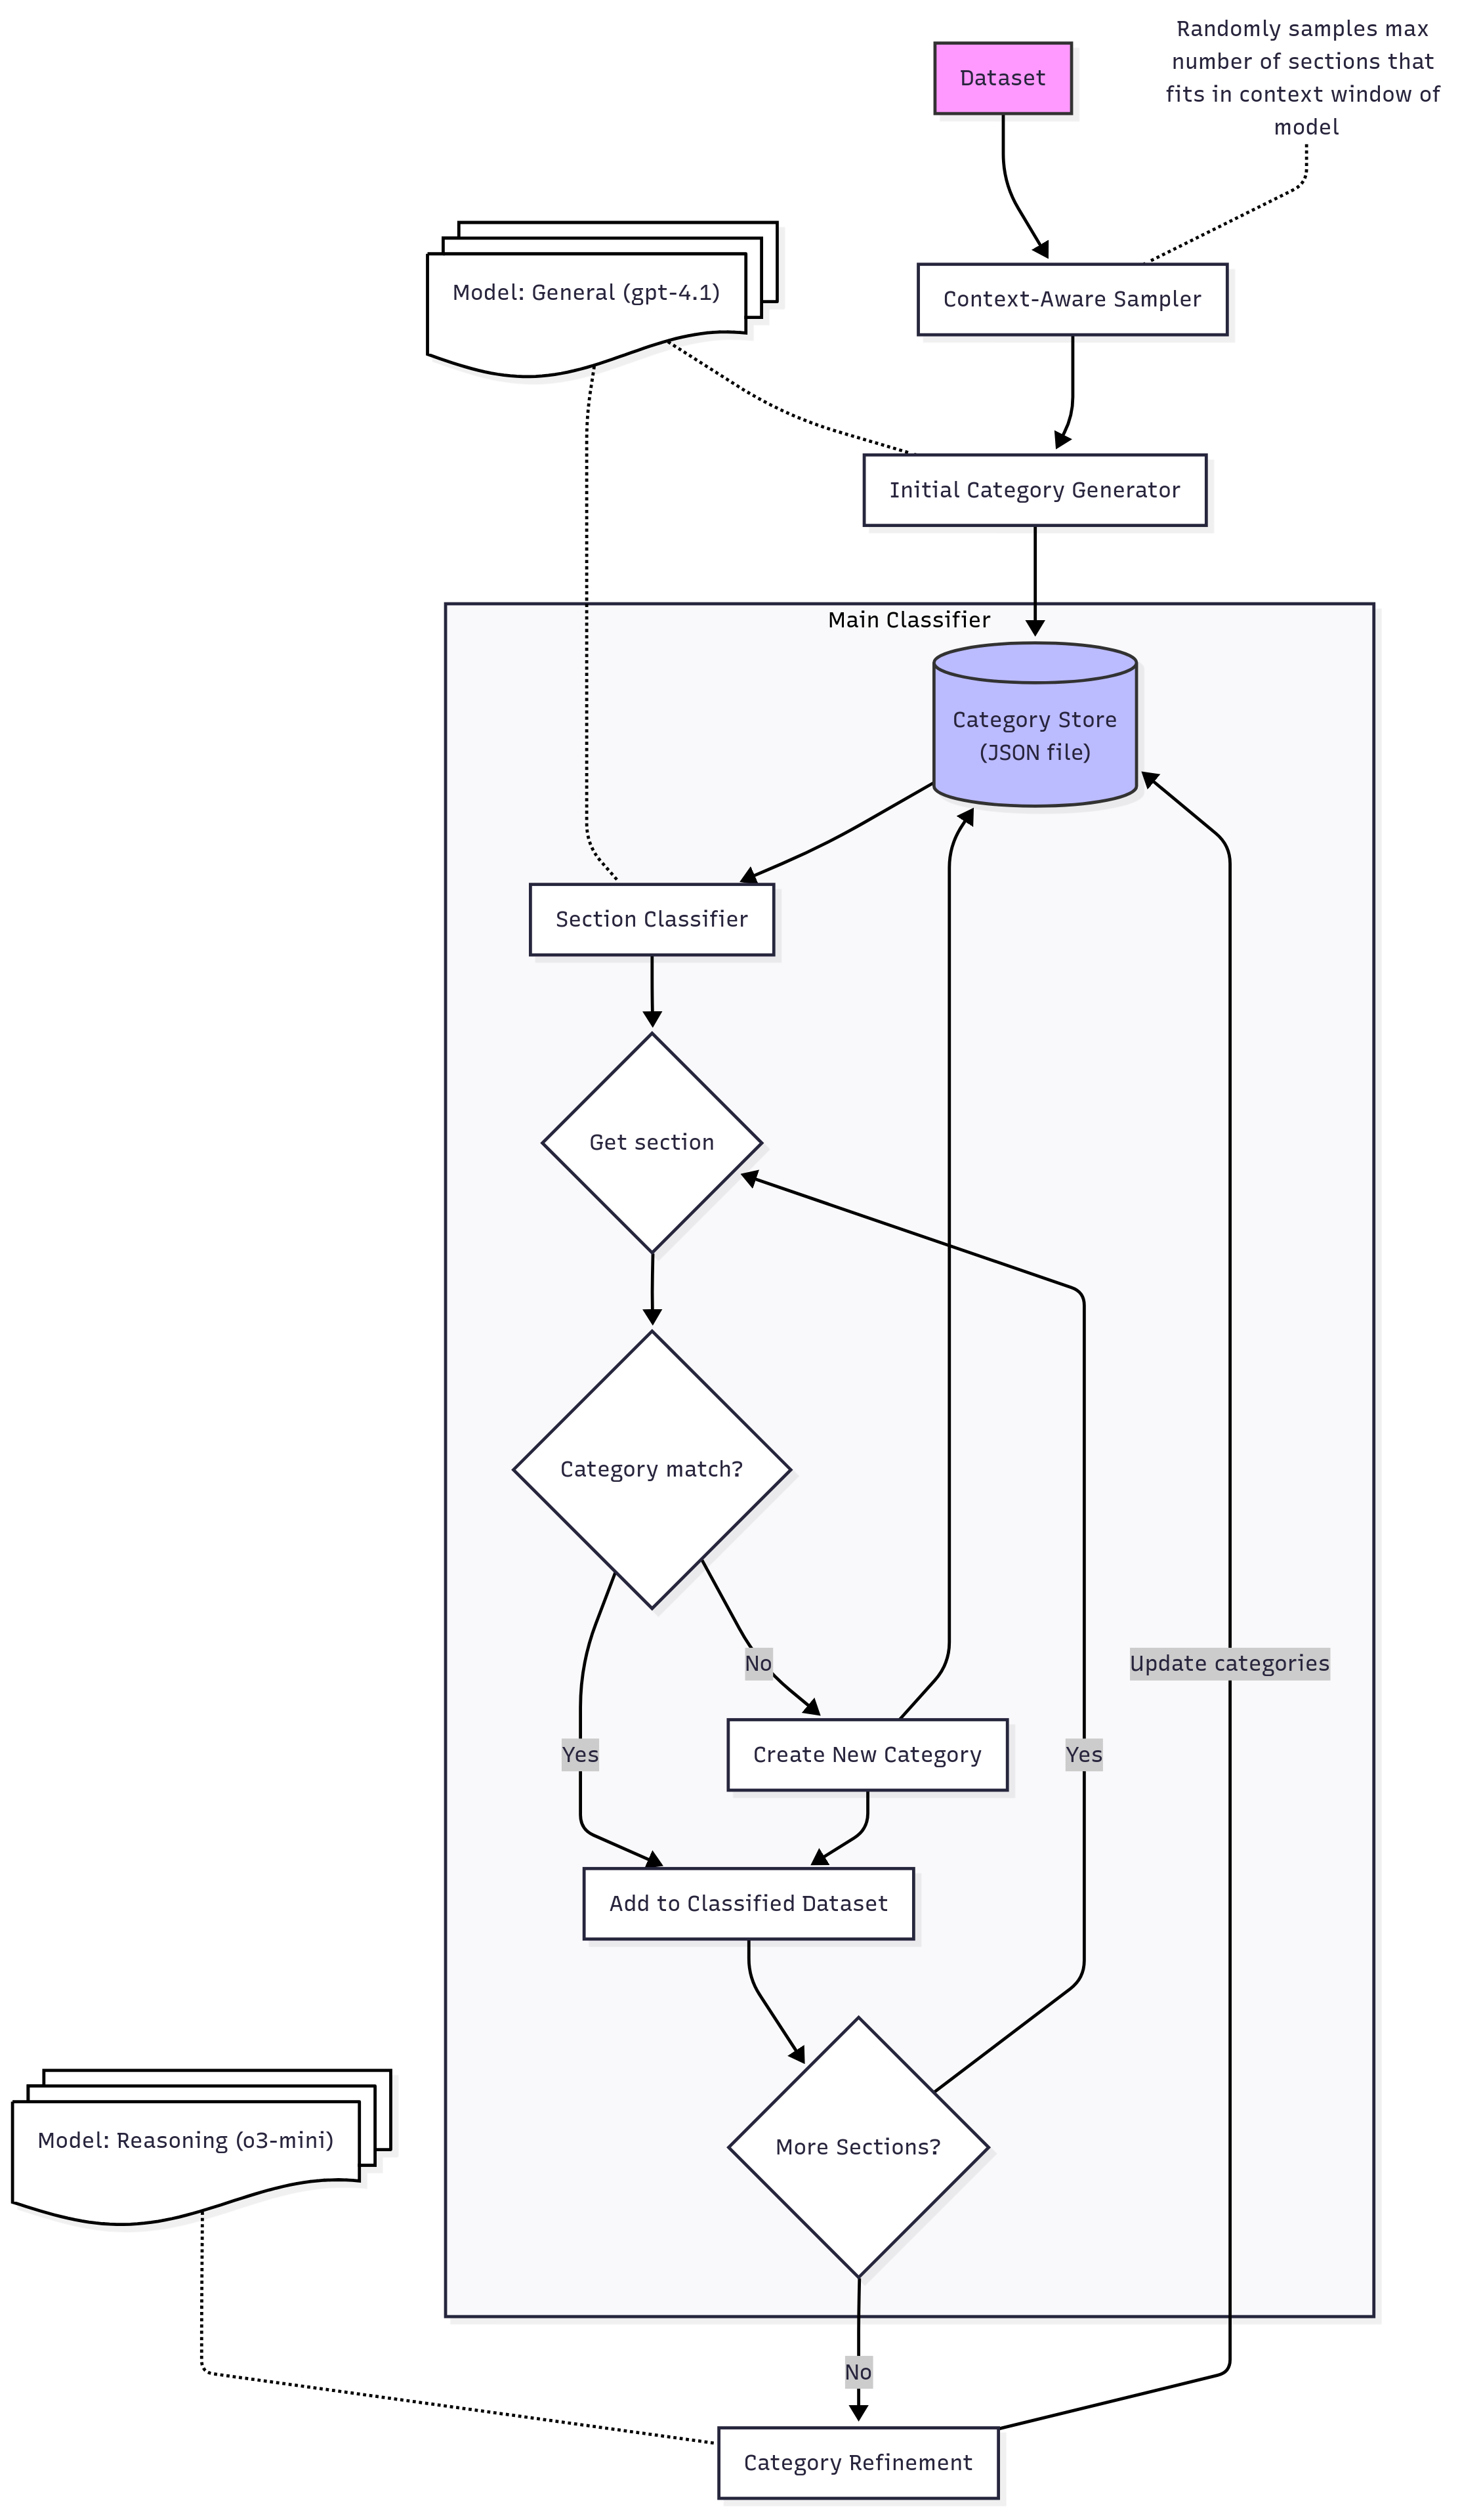
\includegraphics[width=0.7\textwidth]{media/classifier_logic.png}
    \caption{Abstract logic of the iterative LLM classifier.}
    \label{fig:classifier_logic}
\end{figure}

\begin{figure}
    \centering
    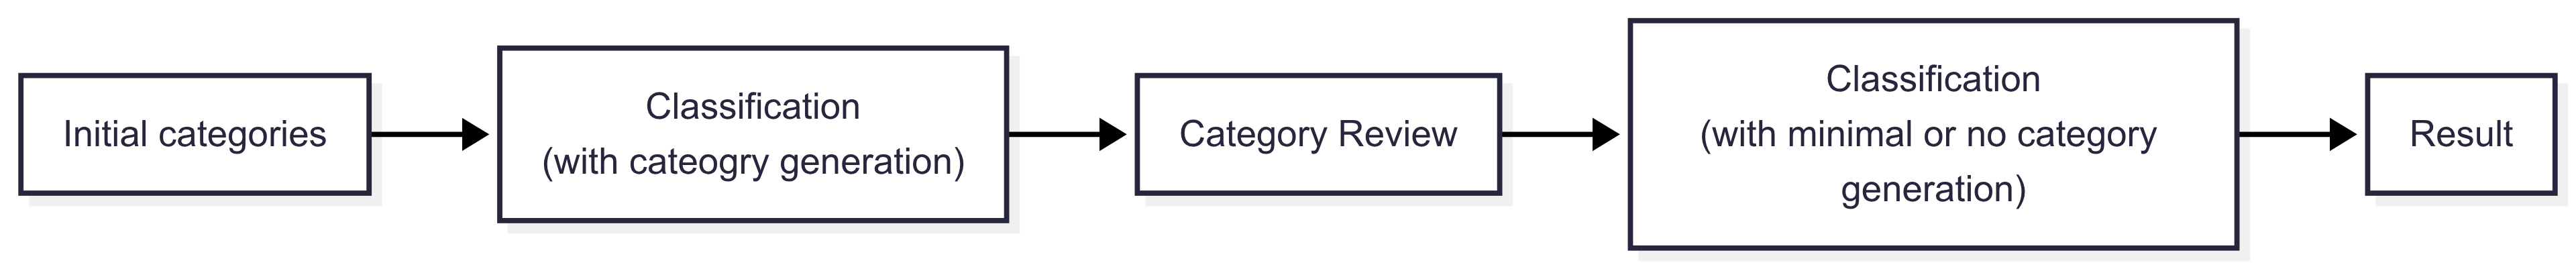
\includegraphics[width=0.7\textwidth]{media/general-workflow.png}
    \caption{General workflow of how we used the classifier to generate results.}
    \label{fig:classifier_workflow}
\end{figure}

\subsubsection{Identifying and Classifying Theoretical Frameworks}

We first applied this workflow to the 589 sections classified as `Theoretical
Framework`. The process generated a fine-grained list of 135 distinct
frameworks. To make this data more interpretable for trend analysis, we ran the
classifier on the framework list itself to group them into six meta-categories
(e.g., \emph{Cognitive, Sociocultural, Social Justice}). Using these
meta-categories, we were able to plot the evolution of theoretical interests in
PRPER over time, as shown in Figure~\ref{fig:theoretical_development}.

\begin{figure}
    \centering
    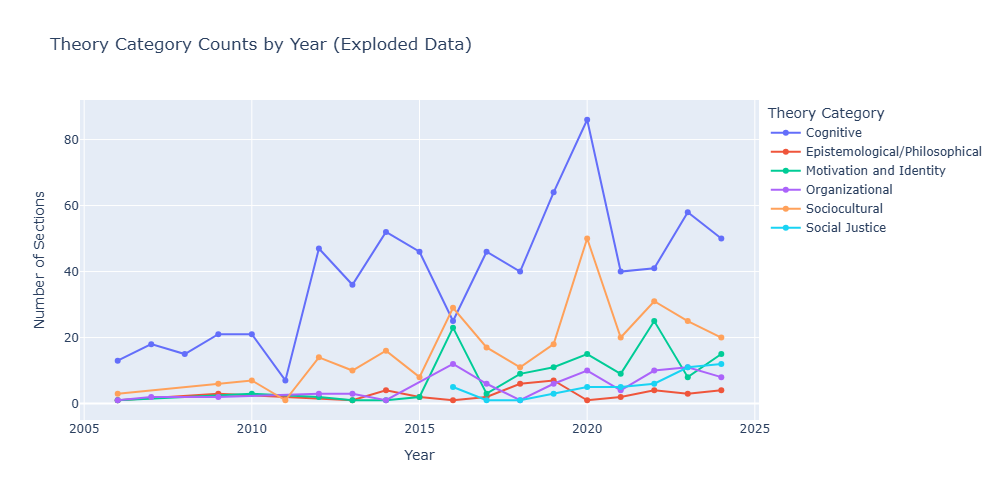
\includegraphics[width=0.7\textwidth]{media/theory_year_exploded.png}
    \caption{Theoretical developments in PRPER over time, grouped by meta-category.}
    \label{fig:theoretical_development}
\end{figure}

\subsubsection{Identifying and Classifying Methods}

We replicated the same process for all sections classified as `Methods`.
As we had no predefined meta-categories for research methods, we used the
classifier's automatic category generation feature to produce an initial list
for review. This allowed us to meta-categorize the identified methods and plot
their development over time.

\subsection{Discussion of the Iterative Classifier}

This iterative, LLM-based approach has several significant advantages. Rather
than relying on a predefined list, the classifier discovers emergent theoretical
and methodological categories directly from the corpus, making it a powerful
tool for large-scale, qualitative discovery. Furthermore, its implemented as a
flexible software framework. The classifier is built upon a set of abstract
Python classes that define the core iterative workflow. This design allows for
easy extension to new tasks; one can create a novel classifier, for example to
identify research questions, simply by inheriting from a base class and
providing new, task-specific prompts. The framework also uses Pydantic models to
ensure that all data exchanged with the LLM is structured and valid. For more
technical details, see the module's documentation.

However, the approach involves practical considerations and trade-offs. The
iterative process, which involves multiple chained calls to an LLM, can incur
monetary costs with APIs. As we noted earlier, running these tasks on powerful,
local open-source models would solve the cost and data privacy issues but
demands notable local computing resources. Furthermore, the "black box" nature
of LLMs means that the reasoning behind category creation is not always
transparent, and the process requires a human-in-the-loop to review and validate
the generated categories for quality and coherence.

A key challenge we noticed, particularly when classifying research methods, was
that the model sometimes struggled to distinguish between the \emph{use} of a
method versus the \emph{discussion} of one. For instance, some articles were
classified as employing both qualitative and quantitative methods. While time
constraints prevented a systematic manual review of these cases, we suspect that
an article can \emph{use} one approach while contrasting it with another; i.e.
the LLM can struggle to distunguish between \emph{use} and \emph{discussion} of
a method. This suggests the `gpt-4o-mini` model, while efficient, can lack the
nuance to grasp this contextual distinction. We hypothesize that using a more
powerful model could mitigate this issue, as it may be better at discerning an
author's primary methodology from the surrounding methodological discussion.

Despite these considerations, this method enables a novel form of automated
literature review, allowing for a fine-grained analysis of conceptual trends at
a scale that would be prohibitive to achieve manually.

% !TEX root = rapport_root.tex
\section{Analysis using projections}
The following sections outlines the use of the previously described 2D projection scoring to analyze, classify and interpret patterns among theoretical frameworks published in physics education research, utilzing the ChatGPT-sorted dataset containing $\sim$600 "Theory" sections, divided into $\sim130$ seperate categories.

\subsection{Category Grouping using Centroid Difference Vectors}
\noindent Attempting to divide these $\sim130$ seperate categories into two superordinate classes, we identify two rough overarching categories
\begin{enumerate}
    \item Cognitive, Conceptual and Mathematical Theories.
    \item Critical Theories concerning Social Justice, Identity and related constructs.
\end{enumerate}
Mean embeddings for each were calculated using the frameworks "Philosophy of Science", "Mathematical Modeling", "Conceptual Change Theory", "Cognitive Load Theory" and "Communities of Practice", "Critical Race Theory" and "Sociocultural Identity Frameworks", respectively. Taking the vector difference of these centroids and projecting all samples against it, we see a rough clustering (see \Cref{fig:109}). The right hand side of the plot contains theories such as "Culturally Relevant Pedagogy", "Gender Performativity" and "Quantitative Critical Race Theory", while the left side is mostly inhabited by different conceptual theories such as "Conceptual Blending Theory" and "Conceptual Metaphor Theory", as well as "Measurement Theory", "Epistemic Games" and "Math-Physics Algorithmic Theory". The middle ground is occupied by "Activity Theory", "Argumentation Theory" and "Intellectual Humility Framework" which perhaps do not fit very well into either category.

\begin{figure}%[h]
    \centering
    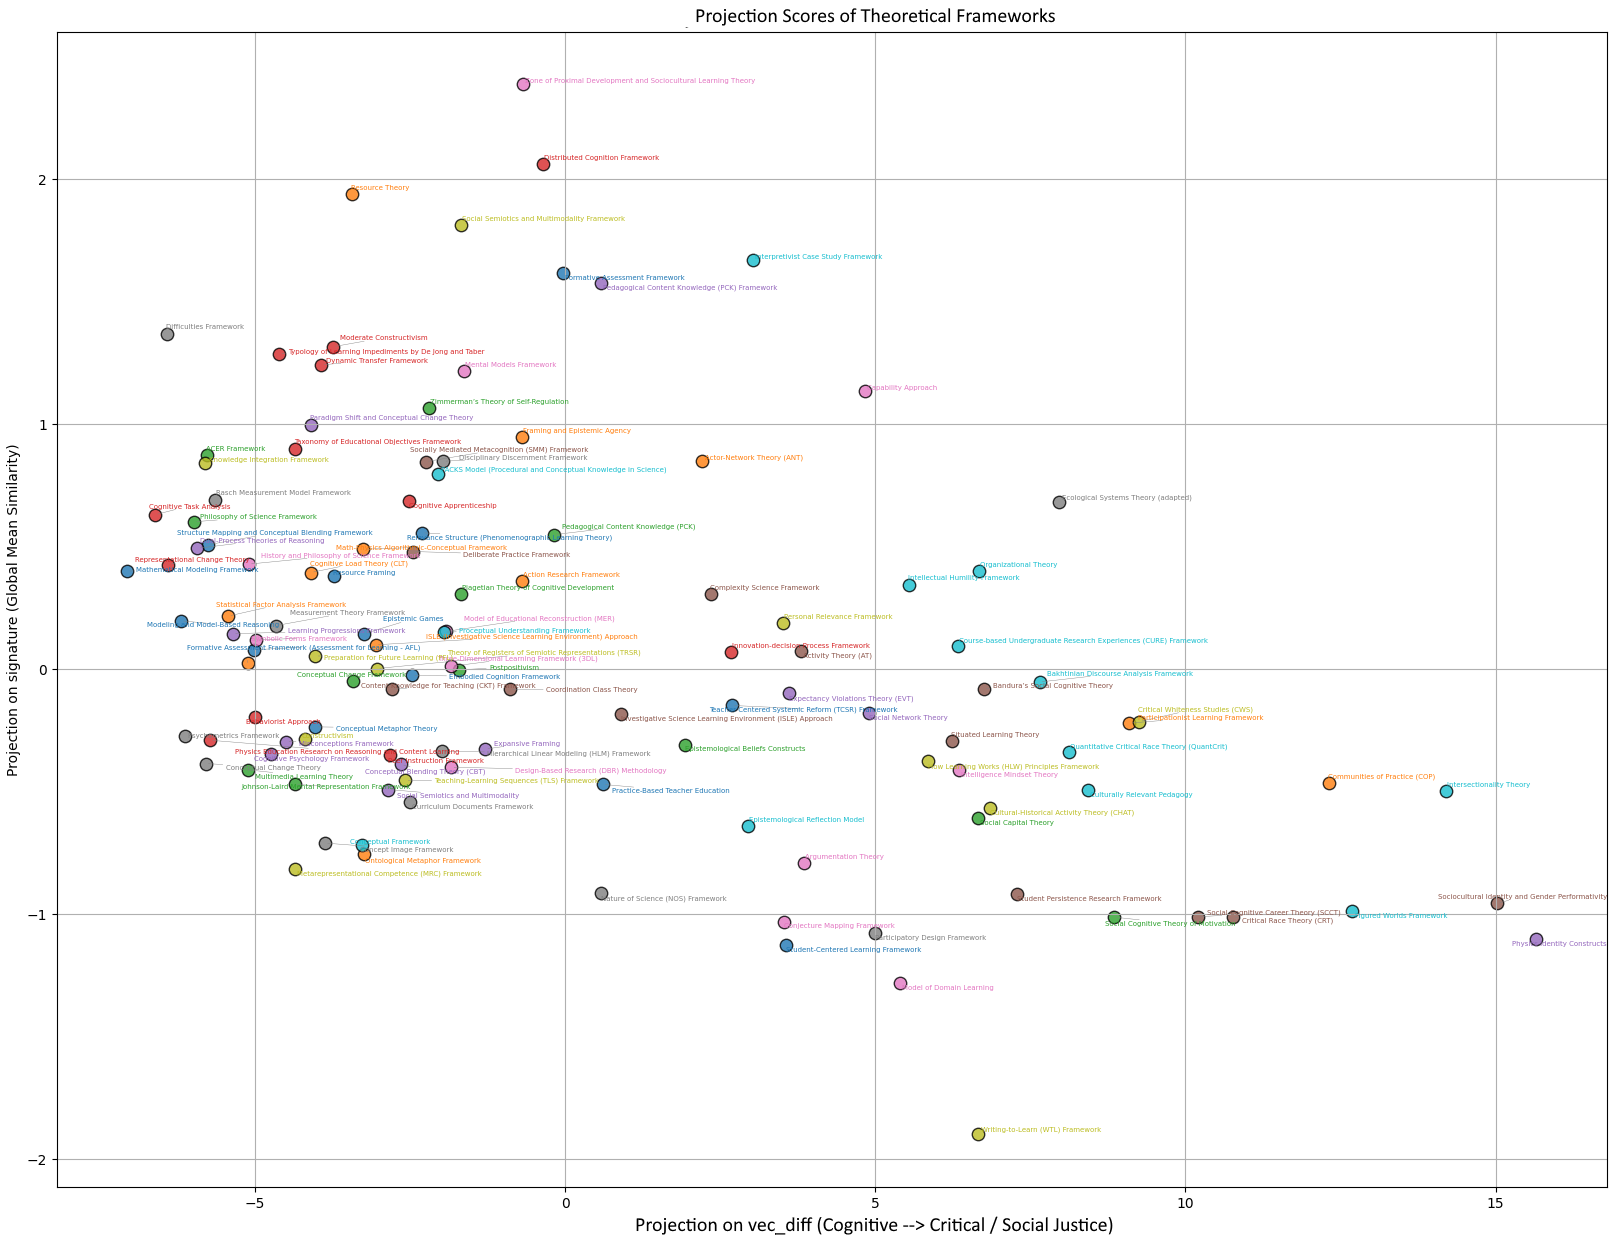
\includegraphics[width=1\linewidth]{media/theoretical_frameworks_socio_cognitive.png}
    \caption{2D projection scores of different theoretical frameworks, projection onto a "Cognitive/Critical" theories difference vector (x-axis) and the global average (y-axis).}
    \label{fig:109}
\end{figure}


In an attempt to make this sorting more rigorous we trained the previously developed projection models on this "Cogntive/Critical" theories difference vector and their respective class means. Applying the resulting classification model to the data, we saw a seemingly logical correlation between the theoretical framework and model classification of it as belonging more to either class 1 or 2 (see \Cref{tab:111}). In future work, it might be interesting to further explore whether a more sophisticated derivation of this method could be used to systematically group data based on certain semantic traits.

\begin{table}[h!]
\centering
\caption{Categorization of Theoretical Frameworks}
\begin{tabular}{|p{7cm}|p{7cm}|}
\hline
\textbf{Class 1 (Cogntive/Mathematical)} & \textbf{Class 2 (Critical/Social)} \\
\hline
Basch Measurement Model Framework & Physics Identity Constructs \\
Cognitive Task Analysis & Writing to Learn Framework \\
History and Philosophy of Science Education & Intersectionality Theory \\
Statistical Factor Analysis Framework & Sociocultural Identity and Gender Performativity \\
Constructivism & Social Cognitive Career Theory \\
Resource Framing & Student Persistence Research Framework \\
Cognitive Apprenticeships & Bandura's Social Cognitive Theory \\
Framing and Epistemic Agency & Social Capital Theory \\
Mathmatical Modeling Framework & Cultural-Historical Activity Theory \\
Multimedia Learning Theory & Quantitative Critical Race Theory \\
\hline
\end{tabular}
\label{tab:111}
\end{table}
\noindent (see notebook '2D\_projection\_space.ipynb' for implementation and further details.)
\subsection{Identifying Temporal Patterns}
Focusing in on specific theoretical frameworks, we attempt to identify temporal patterns by taking the mean embedding of all theories in the first and last year of publishing, and projecting all samples on the difference of the means. Looking at \Cref{fig:110} and \Cref{fig:111}, this approach does not seem to capture any clear linear development of the frameworks over time. While theories published in the same year seem to cluster together, the clusters jump sporadically around the x-axis from year to year rather than follow a clear incremental path from left to right over time (compared to \Cref{fig:108}). This could perhaps indicate that theories are developed in an irregular, unpredictable fashion, rather than a continuous incremental evolution. This being said, a lot of information is lost while projecting the embeddings, and it is entirely possible that a better suited difference vector could reveal a clearer pattern or trajectory.
\begin{figure}%[h!]
    \centering
    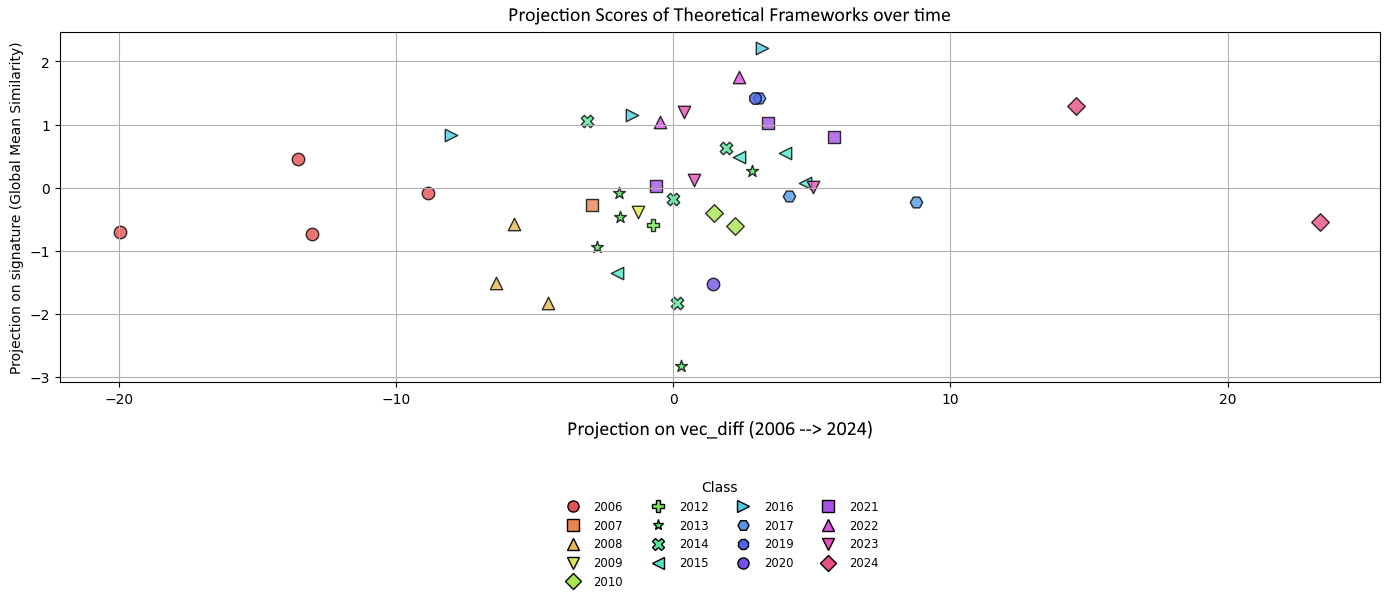
\includegraphics[width=.9\linewidth]{media/resource_framing_temporal.png}
    \caption{Projection scores of all theories classified as "Resource Framing", with 'vec\_diff' being vector difference between mean of years 2024 and 2006.}
    \label{fig:110}
\end{figure}

\begin{figure}%[h!]
    \centering
    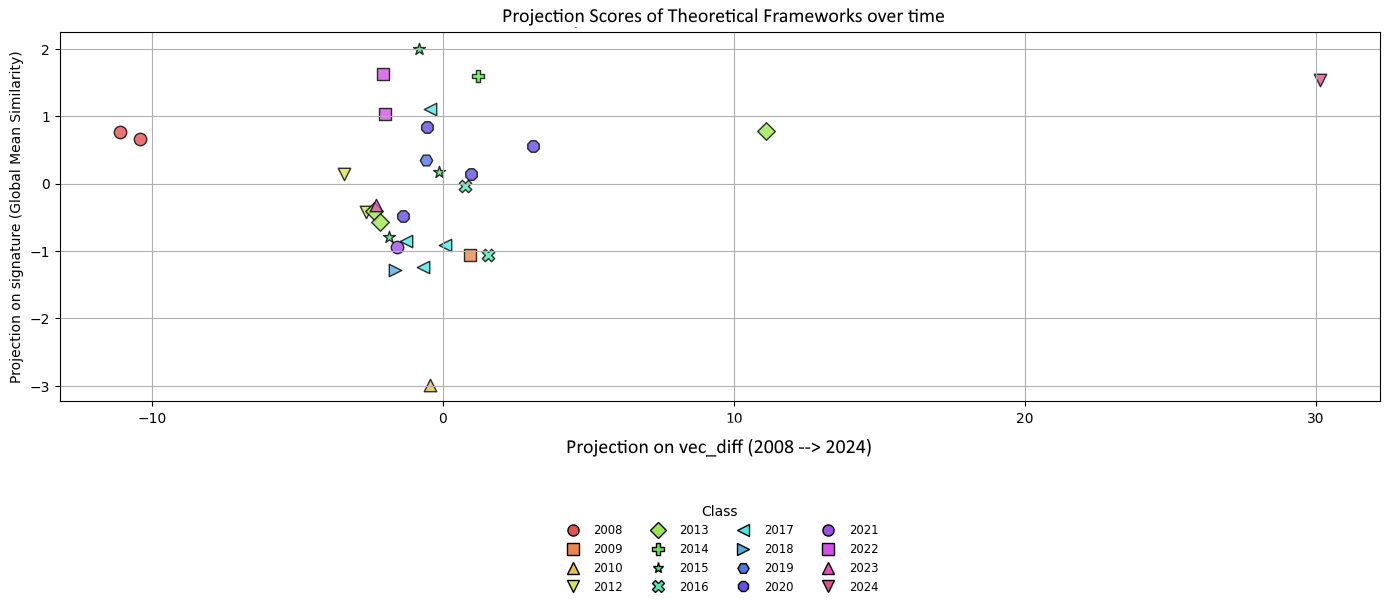
\includegraphics[width=.9\linewidth]{media/modeling_temporal.png}
    \caption{Projection scores of all theories classified as "Modeling and Model-based reasoning", with 'vec\_diff' being vector difference between mean of years 2024 and 2008.}
    \label{fig:111}
\end{figure}

\subsection{Exploring semantic correlations with article citation performance}

Using SemanticScholars API to retrieve citation counts for all the theoretical frameworks, we also attempted to look for correlations between semantic properties and average citations/yr. Dividing the theoretical frameworks into eight quantiles ranging from least to most average citations per year and projecting onto a difference vector based on the means of the highest and lowest quantiles (\Cref{fig:112}), we were unable to find any patterns or general seperation.


\begin{figure}
    \centering
    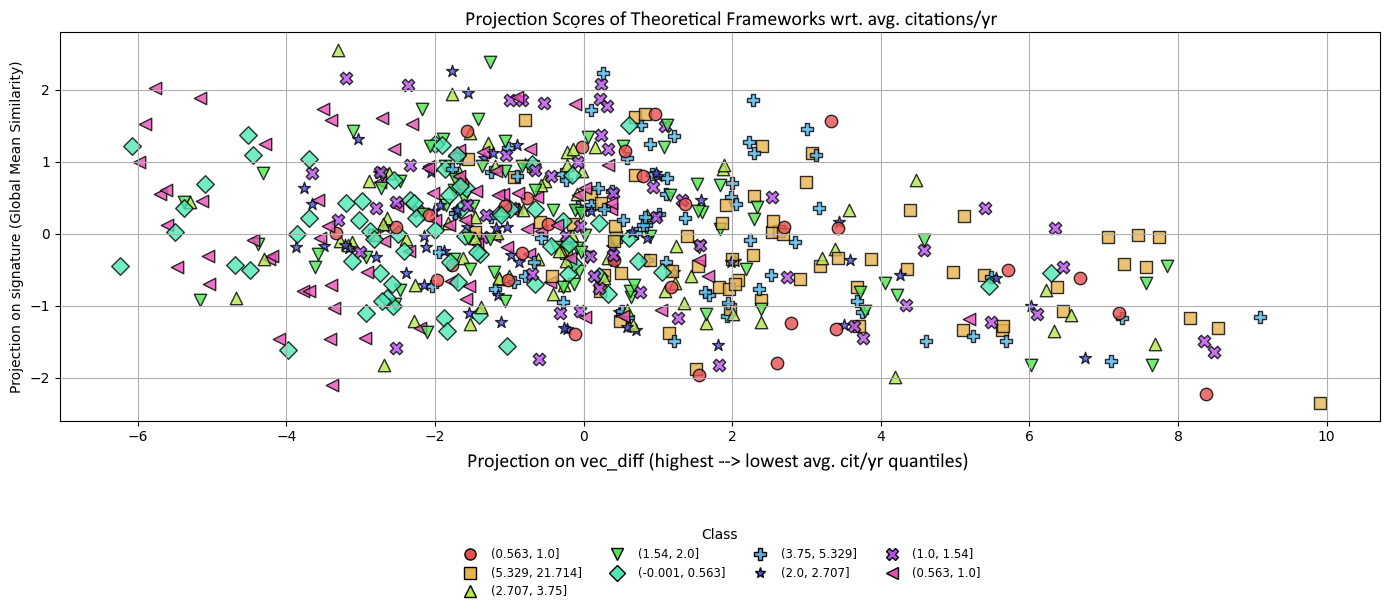
\includegraphics[width=.9\linewidth]{media/avgcityr_all.png}
    \caption{Projection scores of all theories onto difference vector between top and bottom 1/6 quantile of citations per year (x-axis) and global average embedding (y-axis). Points are labeled by their respective citations/year interval.}
    \label{fig:112}
\end{figure}
 We did however see a clear seperation between the lowest and highest citation quantiles (\Cref{fig:113}). Training our MLP projection model on this binary problem using a 0.7/0.3 train-test-split, it performs with an accuracy of $\sim$0.76. This indicates that there exists some semantic characteristic differentiating high- and low-traction academic papers.
\begin{figure}
    \centering
    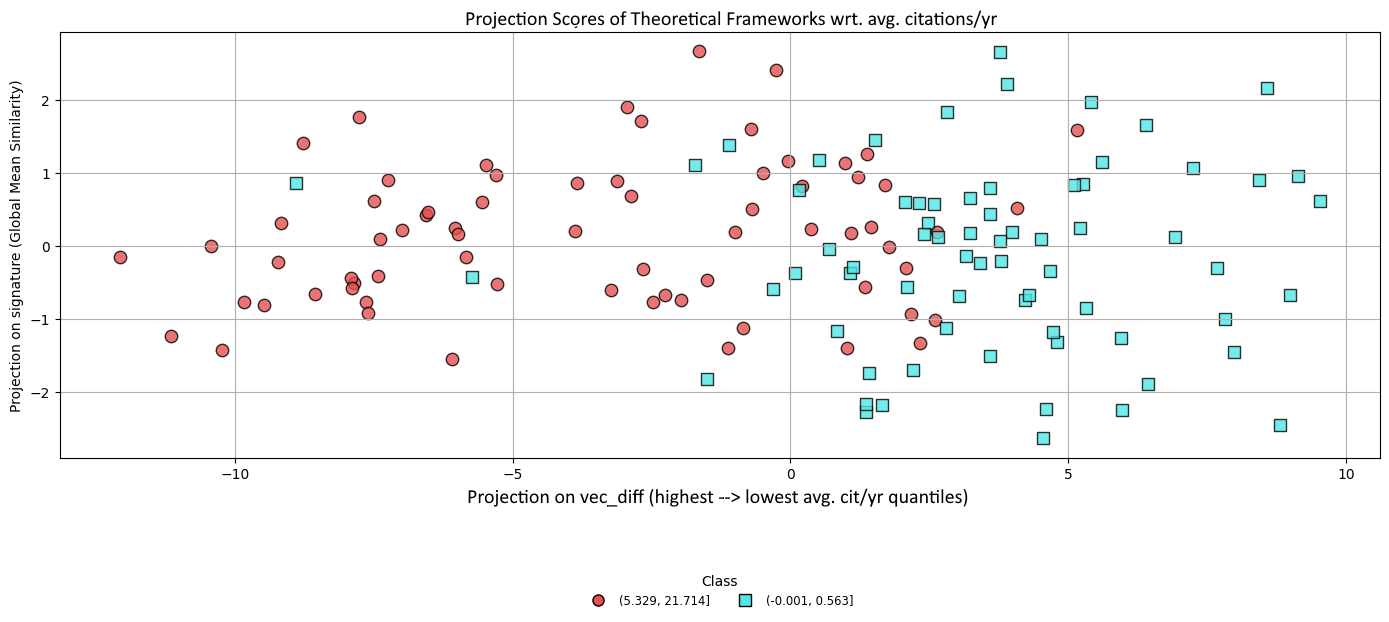
\includegraphics[width=.9\linewidth]{media/avgcityr_binary.png}
    \caption{Projection scores of all theories onto difference vector between top and bottom 1/6 quantile of citations per year (x-axis) and global average embedding (y-axis). Points are labeled by their respective citations/year interval. Here we only include points belonging to the bottom and top quantile.}
    \label{fig:113}
\end{figure}
Attempting to determine whether this semantic difference is related to the underlying nature of the theoretical frameworks, we again project the samples onto the aforementioned "Cognitive/Critical" difference vector, labeling each point by their citation performance. Looking at \Cref{fig:114}, there does not seem to be a particularly noticable crowding of either low- or high-citation papers on either the "social/critical" or "cognitive/mathematical" side, perhaps indicating that this differentiating semantic property is not dependent on theoretical orientation. Of course, this type of "visual" analysis is very "hand-wavey" and lacking in rigour, so these results should be taken with many a grain of salt.
\begin{figure}
    \centering
    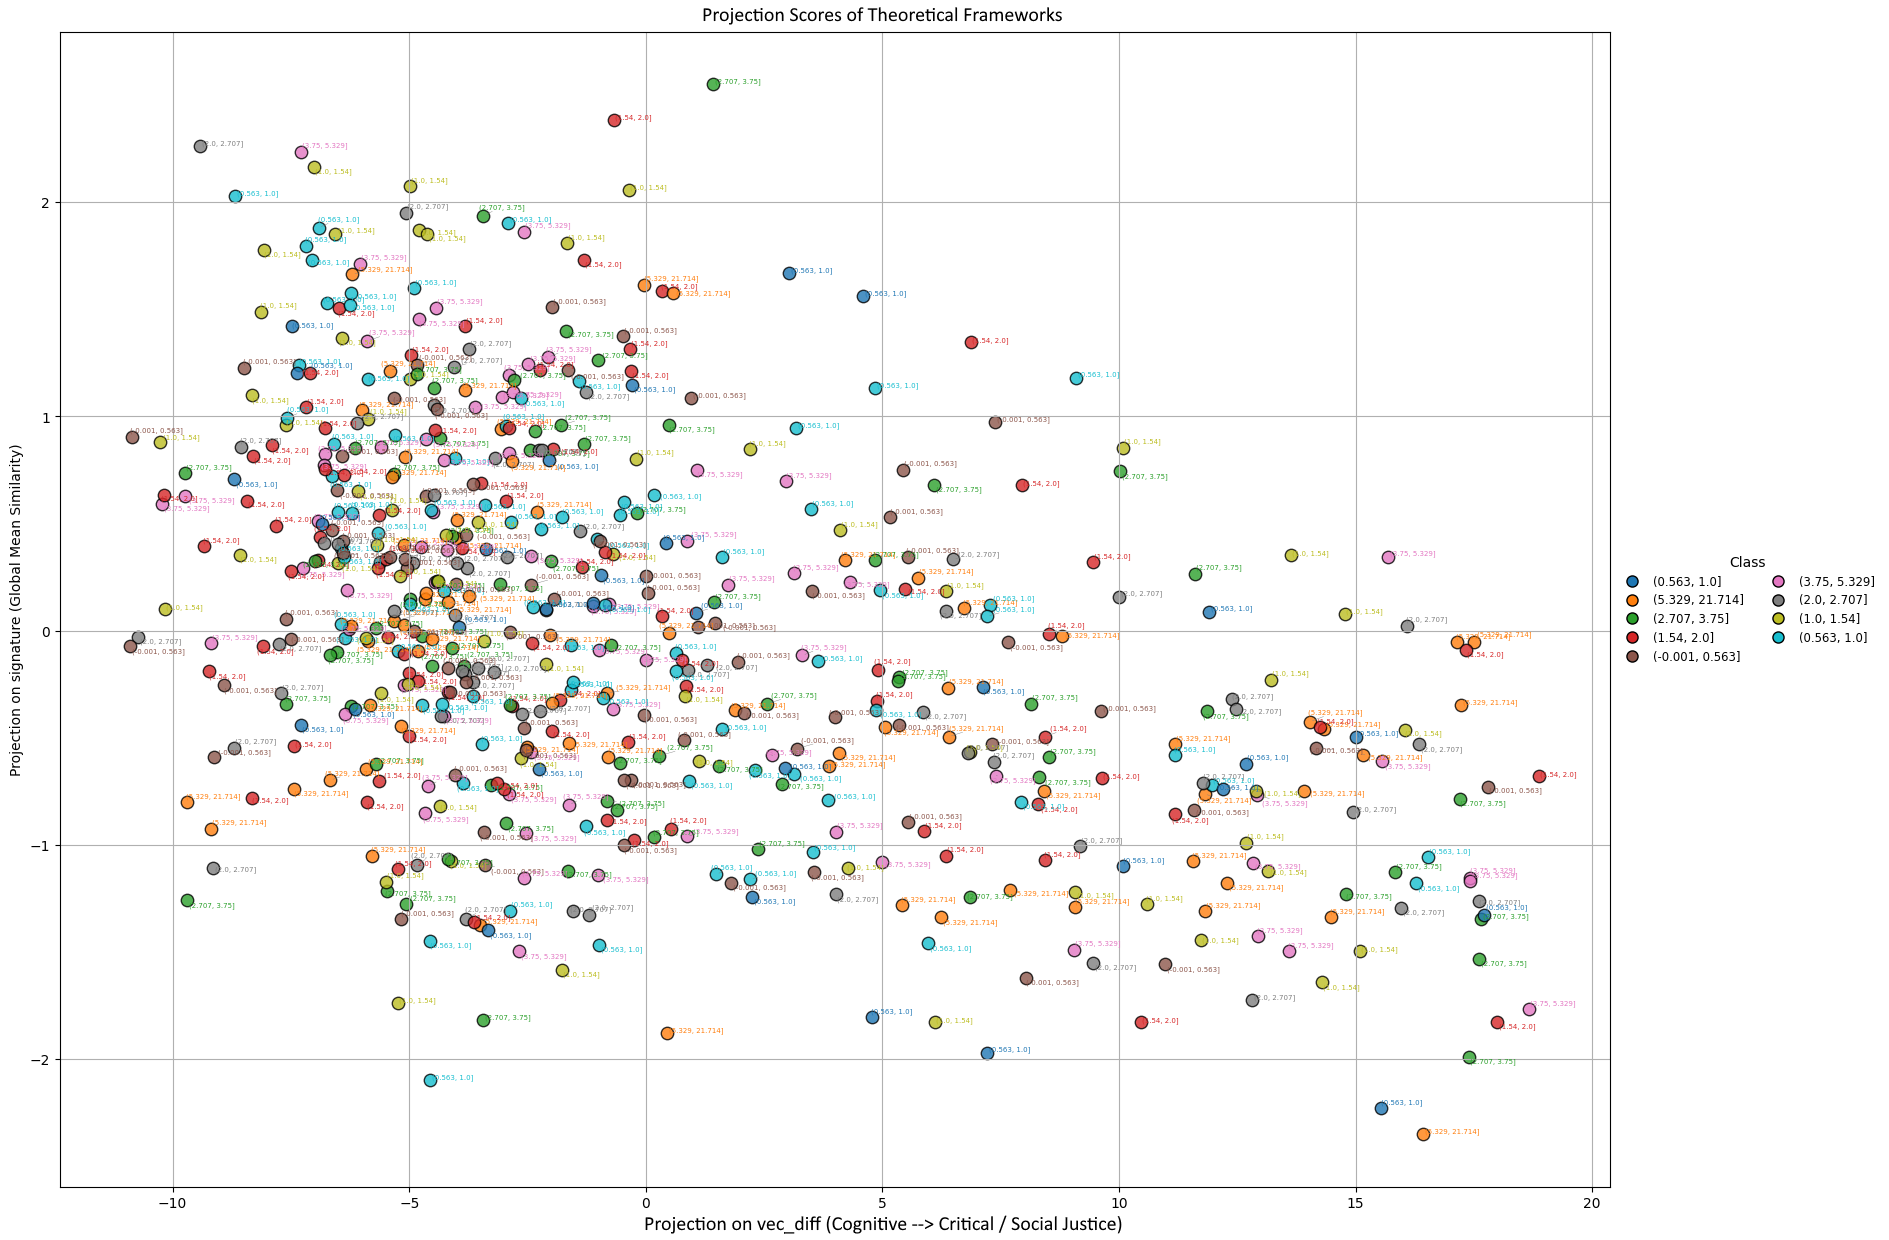
\includegraphics[width=1\linewidth]{media/cogn_crit_proj_citations.png}
    \caption{2D projection scores of theoretical framework embeddings onto "Cogntive/Critical" difference vector (x-axis) and global average (y-axis). The points are labeled according to their citations/year quantile.}
    \label{fig:114}
\end{figure}

\subsection{Discussion and Future Work}

This type of projection-based analysis, primarily centered on vector differences between mean embeddings, is conceptually intuitive and easy to implement. The general idea of substracting mean centroids to produce customized interpretable axes seems to have some merit, yielding results that align with plausable groupings. The low computational cost and high data-efficiency allows for rapid iteration and testing of different grouping hypothesis. The method is also very generalizable, and swapping the constituent centroids of the difference vector immediately changed the result sample layout in understandable ways. This flexibility could make it a useful exploratory tool.

However, the success of this method hinges almost entirely on the usefulness of the chosen difference vector. Selecting representative anchors for each conceptual pole is also a subjective process and could easily bias the outcome. Furthermore, semantic centroids flatten all internal variation within a category, and projecting all embeddings down into a 2D space may be conceptually easy to interpret, but this comes at the cost of signficant information loss that is difficult to account for. And while the results may appear conceptually straightforward, this can be misleading; these geometric operations occur in highly abstract, high-dimensional spaces, and their outcomes are not always as semantically meaningful as they might initially seem. Lastly, unlike clustering or supervised classification where evaluation metrics can guide interpretation, projection maps rely heavily on visual inspection. This makes it difficult to rigorously assess what a pattern means, or whether it’s meaningful at all.


While this analysis demontrates the potential of the projection-based semantic approach, it raises many questions and directions for future study. Further work is required to identify what the projection space captures in general. While the method is efficient and visually intuitive, interpretability of the axes remains a challenge. Although the citation difference vector successfully seperates highly and sparsely cited papers, its semantic signficant remains unclear; does it reflect alignment with theoretical paradigms, or is it more sensitive to shallow lexical and grammatical properties? Can any insights be derived from the relationship between x- and y-axes? Shedding light on these areas may also aid in the identification of temporal difference vectors that more clearly capture patterns over time. Investigating how different pre-trained models, embedding granularities, or normalization techniques affect projection behavior may also help interpret the semantic dimensions being encoded.


Developing or utilizing more rigorous inspection tools is also essential. Currently the analysis relies solely on visual inspection of plots, which is prone to inaccuracy and subjective bias. It would also be interesting to explore whether similar tools, in conjunction with a more sophisticated derivation of this method, could be used to systematically group data based on certain semantic traits. This would perhaps allow for other interesting prospects, such as the identification of emerging theoretical frameworks or under-cited but semantically novel work.

\section{Conclusion}

This report set out to address a key limitation in the computational analysis of scientific literature: the loss of nuance when treating entire articles as single data points. We developed and evaluated a complete workflow for performing a fine-grained, section-level analysis of the PRPER corpus, demonstrating the feasibility and value of this approach.

Our initial exploration confirmed that while a section-level approach is necessary, it is also challenging, as the thematic signal of an article often dominates the more subtle rhetorical signal of its sections. To overcome this, we compared several supervised classification models. We found that a Large Language Model using an external API achieved the highest accuracy at $\sim$90\%, while a novel, projection-based MLP classifier offered a strong and computationally efficient local alternative ($\sim$80\%), outperforming a fine-tuned SciBERT model ($\sim$77\%).

Using the most accurate classifications, we pioneered a novel, iterative LLM-based method capable of discovering and categorizing specific theoretical frameworks and research methods directly from the text. This technique successfully mapped the conceptual evolution of the PRPER journal over two decades, showcasing its potential as a powerful tool for automated, data-driven literature reviews.

This work is not without limitations. The classification task is complicated by the inherent ambiguity of section boundaries, and the iterative analysis method requires significant computational resources and human-in-the-loop validation. Future work should focus on applying this workflow to other research corpora and refining the iterative classifier with more powerful models to better distinguish between the "use" and "discussion" of a concept. Further investigation into the semantic axes discovered through projection-based analysis could also yield more rigorous tools for interpreting the conceptual landscape of a scientific field.

\printbibliography[title={Bibliography}]

\end{document}


